\chapter{Theoretical Background}\label{chapter:theoretical_background}

This chapter establishes the theoretical foundations that underpin this research, organized into four sections, serving as a leveling ground for the reader. In the \autoref{sec:ag_contextualization} section, essential concepts of agricultural \ac{RS} are presented, including a review of vegetation indices, Earth observation satellites, and a review of public datasets available in the literature. Next, in the \autoref{sec:ml_contextualization} section, the principles of \ac{ML} are discussed, ranging from classic \ac{SL} models to state-of-the-art \ac{DL} architectures, such as Transformers and post-Transformer architectures. The \autoref{sec:ssl_contextualization} explores \ac{SSL}, detailing contrastive, masked modeling, and hybrid techniques widely used to train some of the latest models. Finally, the \autoref{sec:conf_contextualization} section describes the problem of confidence detection in predictions, including anomaly detection.


\section{Agricultural Remote Sensing}
\label{sec:ag_contextualization}

\fromsurvey{\ac{RS} can be defined as the field that studies, from a distance, objects and phenomena \citep{Jensen2014}. Remotely sensed data can be acquired from non-contact sensor systems, such as satellites, planes, and drones. All sensors are based on the study of \ac{EMR} and the ability of individual targets to reflect, absorb, and transmit this \ac{EMR} \citep{Jensen2014, Brandt2009}. According to the authors, there are two main types of sensors: (i) passive and (ii) active. Passive sensors are those that can only receive \ac{EMR}, such as optical and thermal sensors. Active sensors are those that can transmit and receive \ac{EMR}, such as \ac{SAR} and \ac{LiDAR}\footnote{Please refer to Jensen \citep{Jensen2014}.}.}

\fromdatacentricai{Except for \ac{LiDAR} data, remote sensing images are usually stored as raster files, usually in TIFF \citep{poynton1992overview} or NetCDF \citep{rew1990netcdf} formats. The term ``raster'' originally comes from the Latin rastrum, meaning ``rake,'' referring to something that ``sweeps'' a surface. In the context of computer graphics and geotechnology, it has been adopted to describe how digital images are organized in a matrix structure \citep{jensen2015introductory, novo2013sensoriamento}. The adoption of the term is also related to the process of acquiring remote sensing images, which often occurs through line-by-line scanning, similar to a systematic sweeping of the terrain.}

\fromsurvey{\ac{LiDAR} and \ac{SAR} sensors are known to be very useful for remotely sensed data. The former is filling an enormous gap in remotely sensed data: more accurate height variations, i.e. 3D data \citep{wangChallengesOpportunitiesLidar2021}. These 3D data can be used to estimate crops and canopy height, which, in its turn, is used for biomass estimation \citep{riveraLiDARApplicationsPrecision2023}. As for the latter, \ac{SAR}, \cite{liuResearchAdvancesSAR2019} explain that \ac{SAR} \ac{EMR} can penetrate clouds, which enables crop monitoring throughout the year without interference. The authors also stated that \ac{SAR} has been quite useful for crop identification because its backscatter is affected by biomass structure, solid condition and provides improved accuracy when used with different polarizations.}

\fromsurvey{Even though \ac{SAR} and \ac{LiDAR} sensors are extremely useful for remote sensing, they are not yet widely used due to their revisit time, which is lower than optical satellite data \citep{Jensen2014}}, This limitation has been further exacerbated by the reported malfunction of one of the most widely used \ac{SAR} sensors, Sentinel-1B, which became inoperative on December 23, 2021 \footnote{Mission ends for Copernicus Sentinel-1B satellite - \url{https://www.esa.int/Applications/Observing_the_Earth/Copernicus/Sentinel-1/Mission_ends_for_Copernicus_Sentinel-1B_satellite}}, resulting in a significant data gap, particularly in some regions (see Table \ref{tab:context-satellites}). \fromsurvey{Another drawback is that their process is far more complex than optical data. \ac{SAR} data needs to be chosen according to the necessity: the polarization, ascending or descending orbit, single look complex, etc. This data is also provided in \ac{dB}, a logarithmic scale. Besides, \ac{SAR} usually follows the Rayleigh distribution \citep{kuruogluModelingSARImages2004}, unlike most optical data that follow the normal distribution. This indicates preprocessing for \ac{SAR} data, which requires computational effort and specific knowledge for processing it. As for \ac{LiDAR} data, it is a point cloud that needs to be processed into a model to be later used as an input for machine learning models  \citep{riveraLiDARApplicationsPrecision2023}. In a nutshell, both \ac{SAR} and \ac{LiDAR} data are not as easy to process and explain as optical data is.}

\fromsurvey{When it comes to optical sensors, we can study how each target can respond to each size of electromagnetic wave, which usually vary from \ac{VIS} - from 450 to 750 nm - to \ac{NIR} - from 750 to 1300 nm - by its reflectance value. Based on that, researchers could describe the spectral behavior for each target, in a sense that the analyst can distinguish types of land cover (eg. water, vegetation, bare soil) and understand its characteristics \citep{plants12122347}. From these different spectral responses, it is even possible to differentiate crops, as shown in Figure \ref{fig:context_reflectances1}. This Figure presents different patterns for each type of crop (corn, sugarcane, coffee, canola, wheat, tobacco) according to their respective factor of reflectance.}

\fromsurvey{For a thorough observation in Figure \ref{fig:context_reflectances1}, wheat is more easily distinguished from the other crops, once its reflectance is higher for almost all wavelengths, mainly \ac{NIR} and \ac{SWIR}. On the other hand, tobacco can be distinguished better at \ac{VIS}, in wavelengths close to yellow and so forth.}

\begin{figure}[!ht]
    \centering
    \caption{\fromsurvey{Example of spectral behavior of different crops classes.}}
    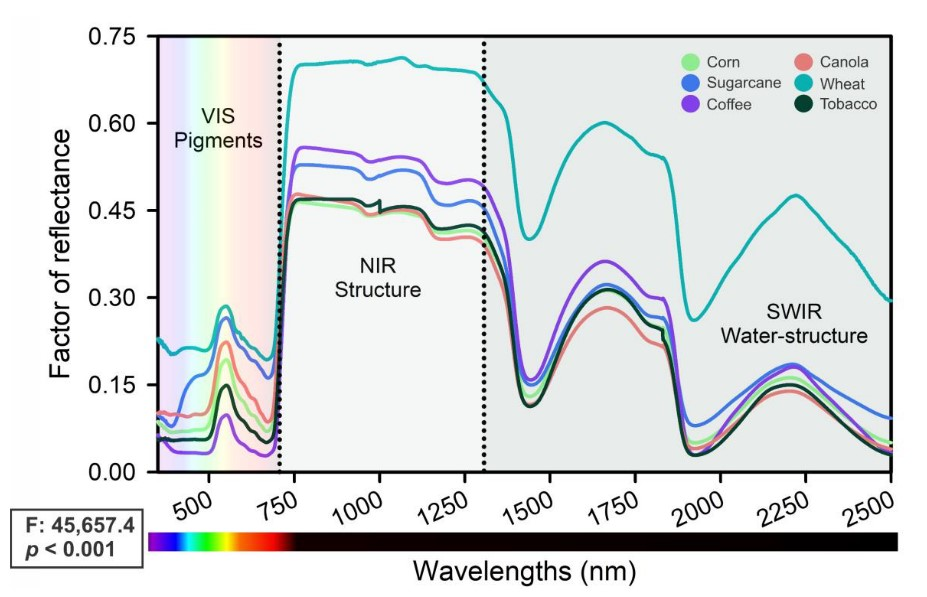
\includegraphics[width=0.95\linewidth]{figures/3_theoretical_background/veg_reflectance.jpg}
    \fignote{ The wavelengths refer to: visible (VIS), near-infrared (NIR) and short-wave infrared (SWIR). Adapted from \cite{plants12122347}}
    \label{fig:context_reflectances1}
\end{figure}

\subsection{Vegetation Indices}

\fromsurvey{From the spectral reflectance, researchers studied methods for better understanding targets and how to discriminate them. They created vegetation indices that, for agriculture, can help analysts to describe vegetation health and age. These indices aim to highlight part of the image with different vegetation cover; they are usually obtained by dividing two spectral bands with high and low reflectance values, respectively \citep{bannari1995review,gao2020remote, ReflectanciaDosMateriais2021}. They are related to spectral estimates for biochemical and biophysical analyses, such as the chlorophyll content and biomass \citep{ndvi1}. Wavelengths approximately between 700 nm up to 1400 nm (\ac{NIR} and \ac{SWIR}) reflect better vegetation than other land covers, such as dry soil and water, while red wavelengths ($\approx$ 660 nm) do not \citep{Jensen2014}.}

\fromsurvey{Some of the most used indices are \ac{NDVI} \citep{ndvi1}, \ac{EVI} \citep{evi1}, \ac{EVI2} \citep{evi2} and \ac{NDYI} \citep{ndyi1} As previously mentioned, all of them consider bands with high reflectance and low reflectance, respectively. \ac{NDVI} was one of the first indices used in \ac{RS}, using red reflectance values ($\rho_{red}$) and \ac{NIR} ($\rho_{NIR}$); it is presented in Equation \ref{eq:ndvi}. This index is extensively used for agriculture, and it has proven to indicate start of seasons and concern for field assessments \citep{FAOfoodandagricultureorganizationoftheunitednationsGuidelinesUseRemote2018}. On the other hand, \ac{EVI} uses the blue reflectance  ($\rho_{blue}$) together with aerosol resistance ($C_1$ and $C_2$) and canopy background ($L$); it is adjusted not to saturate in high-density canopy cover (Equation \ref{eq:evi}). \ac{EVI2} adjusted \ac{EVI} to only two bands, and the authors state that there is no statistical difference between them. As can be seen, if $L=0$, then \ac{EVI2} is very similar to \ac{NDVI}. \ac{EVI} and \ac{EVI2} are used. In general, \ac{NDVI} usually highlights crop flourishing and indicates the amount of humidity in the parcel. On the other hand, \ac{NDYI}, \ac{EVI} and \ac{EVI2} are used to highlight and understand vegetation peaks of crops and differentiate dense structures.}


\begin{equation}
\label{eq:ndvi}
    NDVI = \frac{\rho_{NIR} - \rho_{red}}{\rho_{NIR} + \rho_{red}}
\end{equation}

\begin{equation}
\label{eq:evi}
        EVI = 2.5 \frac{\rho_{NIR} - \rho_{red}} {L + \rho_{NIR} + C_1\rho_{red}-C_2\rho_{blue}}
\end{equation}

\begin{equation}
\label{eq:evi2}
    EVI2 = 2.5 \frac{\rho_{NIR} - \rho_{red}}{\rho_{NIR} + \rho_{red} + L}
\end{equation}

\begin{equation}
\label{eq:ndyi}
    NDYI = \frac{\rho_{green} - \rho_{blue}}{\rho_{green} + \rho_{blue}}
\end{equation}

\subsection{Earth Observation Satellites}
\label{sec:context_satellites}

\fromsurvey{Since the 1970s, earth observation satellites have been developed to monitor target tasks with specific spectral responses, including vegetation, soil, water, and climate variables. The United States' \ac{NASA} initiated the Landsat program in 1972, creating the longest continuous global land observation record \citep{masek2020,wulder2022}, while its \ac{EOS} expanded capabilities with sensors like \ac{MODIS} and \ac{ASTER} \citep{nasa2020}. The \ac{ESA} developed the Copernicus program with its Sentinel satellite series (2014-present) for open global monitoring \citep{esa2021}, building on earlier ERS and Envisat missions \citep{attema2007}. China's CNSA (China National Space Administration) deployed the Gaofen series (2013-present) and collaborated with Brazil's \ac{INPE} on the \ac{CBERS} program (since 1999) \citep{li2022,lino2000cbers}, with Brazil later launching its first independent satellite Amazonia-1 in 2021 \citep{amazonia2021}. France's \ac{CNES} pioneered commercial high-resolution imaging through \ac{SPOT} (1986-2012) and Pleiades (2011-present) satellites \citep{spot2012,gleyzes2012pleiades}, while India's \ac{ISRO} established regional monitoring via its \ac{IRS} program (1988-present) \citep{navalgund2007}. Also, \ac{JAXA} has missions such as the \ac{ALOS}, a program started in 2006, aiming to provide data for environmental and resource sciences.}


\fromsurvey{
Most EO optical satellites feature specific spectral bands, called \textbf{spectral resolution} \citep{jensen2016}, for different wavelengths:
\begin{itemize}
    \item \textbf{Blue} ($\approx 450-520$ nm),
    \item \textbf{Green} ($\approx 520-600$ nm),
    \item \textbf{Red} ($\approx 630-690$ nm),
    \item \textbf{Near-infrared} (NIR, $\approx 760-1300$ nm),
    \item \textbf{Shortwave infrared} (SWIR, $\approx 1550-1750$ nm and $\approx 2080-2350$ nm).
\end{itemize}}

\fromsurvey{Another crucial aspect of all kinds of remote sensing data is the \textbf{spatial resolution} (the length of one pixel side), classified as:
\begin{itemize}
    \item \textbf{\Acf{VHR}}: $\leq$ 2 m (e.g., WorldView-4),
    \item \textbf{\Acf{HR}}: 2-10 m (e.g., Sentinel-2),
        \item \textbf{\Acf{MR}}: 10-100 m (e.g., Landsat-9),
        \item \textbf{\Acf{LR}}: $\geq$ 100 m (e.g., MODIS) \citep{belward2015}.
\end{itemize}}

\fromsurvey{Also, a critical parameter is the imaging frequency for a given area \citep{wulder2019}, called \textbf{temporal resolution} or \textbf{revisit time}.}

\fromsurvey{The Earth observation data ecosystem includes significant contributions from private companies such as Planet, Maxar, and Airbus, which operate constellations from low up to high-resolution satellites \citep{planet2023,maxar2022,airbus2021}. While these commercial systems provide valuable capabilities for specific applications, our study focuses exclusively on publicly available datasets from programs like Landsat  - \ac{NASA}/\ac{USGS} -  and Sentinel (\ac{ESA}), which offer long-term, research-friendly, open data policies essential for scientific research and global environmental monitoring \citep{masek2020,esa2021}. This emphasis on open data ensures reproducibility and equitable access to Earth observation information across the scientific community. In this direction, some recent initiatives like the \ac{BDC} and \ac{AGDC} simplified \ac{EO} data access by providing easy-to-consume, analysis-ready multitemporal and multisensor data cubes \citep{camara2020,giuliani2020earth}.}

\fromsurvey{Table \ref{tab:context-satellites} summarizes the main satellites referenced in this review, with consolidated information from the \textbf{eoPortal}\footnote{\url{https://www.eoportal.org/}} catalog \citep{eoportal2023}.}


\begin{table}[!ht]
\centering
\caption{\fromsurvey{Main satellite missions used by the selected datasets.}}
\label{tab:context-satellites}

\resizebox{\textwidth}{!}{
\begin{tabular}{lllllllllll}
\hline
\textbf{Mission} && \textbf{Launch} && \textbf{Sensor}&& \textbf{\begin{tabular}[c]{@{}l@{}}Spatial\\ Resolution\end{tabular}} && \textbf{\begin{tabular}[c]{@{}l@{}}Spectral\\ Resolution\end{tabular}}&& \textbf{\begin{tabular}[c]{@{}l@{}}Revisit\\ (days)\end{tabular}} \\ \hline
Landsat-1 (L1)*&& 1972&& MSS&& $\sim$80 m&& VIS, NIR&& 18\\ \hline
Landsat-2 (L2)*&& 1975&& MSS&& $\sim$80 m&& VIS, NIR&& 18\\ \hline
Landsat-3 (L3)*&& 1978&& RBV&& \begin{tabular}[c]{@{}l@{}}$\sim$40 m,\\ $\sim$80 m\end{tabular}&& PAN, VIS, NIR && 18\\ \hline
Landsat-4 (L4)*&& 1982&& TM && $\sim$30 m&& \begin{tabular}[c]{@{}l@{}}VIS, NIR,\\ SWIR, Thermal\end{tabular} && 16\\ \hline
Landsat-5 (L5)*&& 1984&& TM && $\sim$30 m&& \begin{tabular}[c]{@{}l@{}}VIS, NIR,\\ SWIR, Thermal\end{tabular} && 16\\ \hline
SPOT && 1986&& \begin{tabular}[c]{@{}l@{}}HRV, HRVIR,\\ Vegetation\end{tabular} && 1.5-20 m&& VIS, NIR&& 2-3 \\ \hline
POES, MetOp&& 1998&& AVHRR&& $\sim$1.1 km&& VIS, NIR, Thermal && 0.5 \\ \hline
Landsat-7 (L7) && 1999&& ETM+ && $\sim$30 m&& \begin{tabular}[c]{@{}l@{}}VIS, NIR,\\ SWIR, Thermal\end{tabular} && 16\\ \hline
MODIS&& 1999&& Terra, Aqua&& \begin{tabular}[c]{@{}l@{}}250 m, 500 m\\ 1 km\end{tabular} && \begin{tabular}[c]{@{}l@{}}VIS, NIR,\\ SWIR, Thermal\end{tabular} && 1-2 \\ \hline
QuickBird-2&& 2001&& Pan, Ms&& \begin{tabular}[c]{@{}l@{}}0.61 m,\\ 2.44 m\end{tabular}&& VIS, NIR&& 3-7 \\ \hline
ALOS && 2006 &&  \begin{tabular}[c]{@{}l@{}}PALSAR (L-band)\\ AVNIR-2 \\ PRISM\end{tabular} && \begin{tabular}[c]{@{}l@{}}7-44 m\\ 10 m \\ 2.5 m\end{tabular} &&  \begin{tabular}[c]{@{}l@{}}HH+HV or VV+VH\\ RGB-NIR \\ PAN\end{tabular} && 46\\ \hline 
GeoEye-1 && 2008&& MS, PAN&& \begin{tabular}[c]{@{}l@{}}0.41 m,\\ 1.65 m\end{tabular}&& VIS, NIR&& 3-5 \\ \hline
WorldView-2(WV2) && 2009&& Pan, Ms&& \begin{tabular}[c]{@{}l@{}}0.46 m,\\ 1.84 m\end{tabular}&& VIS, NIR&& 1.1 \\ \hline
\begin{tabular}[c]{@{}l@{}}Suomi-NPP,\\ NOAA-20\end{tabular} && 2011&& VIIRS&& 375 m && \begin{tabular}[c]{@{}l@{}}VIS, NIR,\\ SWIR, Thermal\end{tabular} && 1 \\ \hline
Landsat-8 (L8) && 2013&& OLI, TIRS&& $\sim$30 m&& \begin{tabular}[c]{@{}l@{}}VIS, NIR, SWIR,\\ Thermal, Cirrus\end{tabular} && 16\\ \hline
Planet && 2013&& PlanetScope&& 3-5 m && VIS, NIR&& 1 \\ \hline
Sentinel-1 (S1)&& 2014&& SAR C-Band && 10 m&& VV, VH, HV&& 12\\ \hline
CBERS-4&& 2014&& \begin{tabular}[c]{@{}l@{}}PAN, MUX,\\ WFI\end{tabular}&& 5-20 m&& VIS, NIR&& 26\\ \hline
GaoFen-2 (GF2)** && 2014&& PAN, MS&& \begin{tabular}[c]{@{}l@{}}1 m,\\ 4 m\end{tabular}&& VIS, NIR&& 5 \\ \hline
WorldView-3 (WV3)&& 2014&& \begin{tabular}[c]{@{}l@{}}Pan, MS,\\ SWIR\end{tabular}&& \begin{tabular}[c]{@{}l@{}}0.31 m,\\ 1.24 m,3.7 m\end{tabular}&& VIS, NIR, SWIR&& 1 \\ \hline
ALOS-2 && 2014 && PALSAR-2 (L-Band) && 10 m && HH+HV or VV+VH && 16\\ \hline
Sentinel-2 (S2)&& 2015&& MSI&& 10-60 m && \begin{tabular}[c]{@{}l@{}}VIS, NIR,\\ SWIR, RedEdge\end{tabular} && 5 \\ \hline
Sentinel-3 (S3)&& 2016&& \begin{tabular}[c]{@{}l@{}}SLSTR,\\ OLCI, SRAL\end{tabular}&& \begin{tabular}[c]{@{}l@{}}300 m,\\ 1 km\end{tabular} && \begin{tabular}[c]{@{}l@{}}VIS, NIR,\\ SWIR, Thermal\end{tabular} && 1-2 \\ \hline
CBERS-4A && 2019&& PAN, MUX && 5-10 m&& PAN, VIS, NIR && 31\\ \hline
Landsat-9 (L9) && 2021&& \begin{tabular}[c]{@{}l@{}}OLI-2,\\ TIRS-2\end{tabular}&& $\sim$30 m&& \begin{tabular}[c]{@{}l@{}}VIS, NIR, SWIR,\\ Thermal, Cirrus\end{tabular} && 16\\ \hline
ALOS-4 && 2024 && PALSAR-3 (L-Band) && 10 m && HH, HV, VV, VH && 14\\ \hline 
\end{tabular}
}
\caption*{\fromsurvey{*Out of order; **Not open access. \\ VIS: Visible; NIR: near-infrared; SWIR: short-wave infrared; PAN: panchromatic; VV, VH, HV are SAR polarizations referring to Vertical-Vertical, Vertical-Horizontal, Horizontal-Vertical, and Horizontal-Horizontal}.}
\end{table}

\subsection{Pre-existing datasets}

\fromsurvey{Datasets play a crucial role in creating a Machine Learning model, mainly for agriculture, once it can contain \textit{in-situ} data or previous knowledge of the region of interest to be created. Both cases are used for field validation; to be more specific, the \textit{in situ} data can retrieve the reflectance information of the target, creating its chart for spectral behavior \citep{Brandt2009} while field knowledge can aid in \ac{LULC} classification. During the dataset search, we did not find any other review article that mapped datasets before from the previous version of this work \citep{mateuzin2024}. Another point is that datasets tend not to generalize well from one region to another, which is related to differences in biomes, topography, climate and agricultural calendars \citep{gadiraju2023remote, kerner2024multi, huber2024leveraging}, although Transfer Learning can be beneficial \citep{gadiraju2023remote, huber2024leveraging, kerner2024multi, khaki2021simultaneous}. For this reason, we point out the importance of mapping as many datasets as possible.}

\fromsurvey{We have searched for all publicly available datasets to date, though in this study we present those considered to be the most important by either number of citations or data size. We divided those datasets into two categories: (i) labeled, created for supervised learning and (ii) non-labeled, used for representation learning, such as Self-Supervised Learning, as well as for generating synthetic data or for unsupervised learning; this second category of datasets has information of general remotely sensed data since we found a lack of agricultural specific unlabeled datasets. Table \ref{tab:context_labeled_datasets} presents a summary of labeled datasets related to agriculture, considering their respective names, applications, and regions of interest, as well as which EO satellites were used. For more information on these datasets (i.e. labeled classes, state-of-the-art methods, evaluation criteria, etc), the readers are referred to the original papers and/or landing pages for each dataset.}

\subsubsection{Labeled Datasets}\label{sec:labeled_datasets}

\fromsurvey{The filters used for selecting the labeled datasets were: (i) we kept all datasets we found of emerging countries; (ii) small datasets or with regions already in other selected datasets were not considered; (iii) datasets merged into other datasets were not considered as well, and, finally, (iv) we considered only the most recent version for each dataset. In addition to that, Table \ref{tab:context_labeled_datasets} mention models based on remotely sensed data, such as ERA5 \citep{ERA5} and ETH-GCHM \citep{mwildRegionalClimateSimulation1996}, which are climate and weather analyzes, as well as Aster \citep{asterdem} and SRTM \citep{srtm} which are elevation models based on satellite radar data. For unlabeled datasets, there were no filters for selecting them, due to their low quantity.}


\begin{table}[!ht] % [!hb]
\centering
\caption{\fromsurvey{Synthesis of Remote Sensing Labeled Datasets.}}
\label{tab:context_labeled_datasets}
\resizebox{\textwidth}{!}{
\begin{tabular}{lllllllllll}
\hline
\textbf{Name} & \textbf{Application}& \textbf{Region} & \textbf{Input data}\\ \hline
3DFGCC* \citep{ji2020learning} & Crop Mapping& China & GF2\\ \hline
AgriSen-COG \citep{selea2023agrisen} & \begin{tabular}[c]{@{}l@{}}Crop mapping,\\ Parcel Delineation\end{tabular}& \begin{tabular}[c]{@{}l@{}}Austria, Belgium, \\ Catalonia, Denmark, \\ Netherlands\end{tabular} & S2 \\ \hline
AI4Boundaries \citep{d2023ai4boundaries} & Parcel Delineation& \begin{tabular}[c]{@{}l@{}}Western Europe, \\ Scandinavia\end{tabular}& S2, Aerial \\ \hline
BreizhCrops \citep{breizhcrops2020}& \begin{tabular}[c]{@{}l@{}}Crop Mapping,\\ Parcel Delineation\end{tabular}& Brittany& S2 \\ \hline
Crop Yield Prediction USA \citep{selea2023agrisen} & Crop Yielding & USA & Pixel level\\ \hline
Cropharvest \citep{tseng2021cropharvest} & Crop Mapping& Worldwide & S1, S2, ERA5, SRTM Elevation \\ \hline
CropNet \citep{fudong:kdd24:crop_net}& Crop Yielding & USA & S2, weather, yielding\\ \hline
DENETHOR \citep{kondmann2021denethor}& \begin{tabular}[c]{@{}l@{}}Crop Mapping,\\ Parcel Delineation\end{tabular}& Germany & S1, S2, Planet \\ \hline
Fields of The World (FTW) \citep{kerner2024fields} & \begin{tabular}[c]{@{}l@{}}Parcel Delineation,\\ Crop Mapping\end{tabular}& Worldwide & S2 \\ \hline
Global dataset of historical yields \citep{iizumi2020global} & Crop Yielding & Worldwide & County \\ \hline
LEM+ \citep{oldoni2020lem+}& Crop Mapping& Brazil& Plot level \\ \hline
PASTIS-HD \citep{garnot2021panoptic} & \begin{tabular}[c]{@{}l@{}}Crop Mapping,\\ Parcel Delineation\end{tabular}& French& S1, S2, SPOT VHR \\ \hline
Purdue Agro-climatic (PAC) \citep{LIU201761} & Crop Yielding & USA Corn Belt & \begin{tabular}[c]{@{}l@{}}Weather, Soil moisture,\\ soil temperature\end{tabular} \\ \hline
S4A \citep{sykas2022sentinel}& \begin{tabular}[c]{@{}l@{}}Crop Mapping, \\ Parcel Delineation\end{tabular} & Catalonia, France & S2 \\ \hline
Sentinel 2 Crop Mapping \citep{gallo2022in_season} & Crop Mapping& Lombardia & S2 \\ \hline
SICKLE \citep{Sani_2024_WACV}& \begin{tabular}[c]{@{}l@{}}Crop Yielding,\\ Crop Mapping,\\ Parcel Delineation\end{tabular} & India & L8, S1, S2 \\ \hline
TimeMatch \citep{nyborgTimeMatchDataset2021} & Crop Mapping& \begin{tabular}[c]{@{}l@{}}Austria, Denmark,\\ France\end{tabular}& S2 \\ \hline
TreeSatAI \citep{astruc2024omnisat}& Crop Mapping (trees)& Germany & S1, S2 \\ \hline
Varda Global FieldID HUB \citep{GlobalFieldID} & Parcel Delineation& Worldwide & Label Only \\ \hline
BEN-MM* \citep{9552024}& LULC & Worldwide& S2\\ \hline
BigEarthNet v2.0 \citep{clasen2024reben}& LULC & \begin{tabular}[c]{@{}l@{}}Central, Western, \\ Southern Europe\end{tabular} & S1, S2\\ \hline
EuroSAT* \citep{helber2019eurosat}& LULC & Europe& S2\\ \hline
Five-Bilion-Pixels \citep{FBP2023}& LULC & \begin{tabular}[c]{@{}l@{}}China, Vietnam, \\ Japan, France\end{tabular} & GF2 \\ \hline
FLAIR* \citep{ign2022flair1}& LULC & French& Aerial, S2\\ \hline
fMoW* \citep{Christie_2018_CVPR}& LULC & Worldwide& QB2, GeoEye-1, WV2 and WV3\\ \hline
fMoW-S2* \citep{congFunctionalMapWorld2022}& LULC & Worldwide& S2\\ \hline
GEO-Bench \citep{lacoste2024geo}& LULC (Benchmark) & Worldwide& S2, L8\\ \hline
GeoZcx \citep{ZHANG2020183}& Change Detection & China& GE Mosaics\\ \hline
HRSCD* \citep{azv7-ta17-20}& Change Detection & France& S2\\ \hline
LEVIR \citep{Chen2020}& Change Detection & USA& GE Mosaics\\ \hline
MillionAID* \citep{9393553}& LULC & Worldwide& Aerial\\ \hline
MMEarth* \citep{nedungadi2024mmearth} & LULC & Worldwide& \begin{tabular}[c]{@{}l@{}}S1, S2, ERA5, Aster DEM,\\ ETH-GCHM\end{tabular} \\ \hline
RS-4M* \citep{wang2024scaling}& LULC & Worldwide& S2, S1, L8/9, Aerial\\ \hline
SAMRS* \citep{wang2024samrs}& LULC & Worldwide& GF2, Aerial \\ \hline
SatlasPretrain* \citep{bastani2023satlaspretrain} & LULC & Worldwide& S2, Aerial\\ \hline
SCD* \citep{yang2020semantic} & Change Detection & China& Aerial\\ \hline
Sen12Flood \citep{sen12flood_dataset} & Flooding & Worldwide& S1, S2\\ \hline
SEN12MS* \citep{schmitt2019sen12ms}& LULC & Worldwide& S2\\ \hline
SYSU-CD \citep{shi21deeply}& Change Detection & China& Aerial\\ \hline
TimeSen2Crop \citep{9408357}& LULC & Austria& S2\\ \hline
FBIS-22M \citep{lavreniuk2025delineateflowfastcountrylevel}& Parcel Delineation & Europe & VHR Sats\\ \hline
\end{tabular}
}
\caption*{*Terabyte sized\\Where, \\GF2, S1, S2, L8, L9 SPOT and Planet refer to EO satellites in Table \ref{tab:context-satellites}; \\Aerial refers to aerial imagery; \\GE Mosaics refer to imagery mosaics from Google Earth}
\end{table}

\subsubsection{Unlabeled Datasets}

\begin{table*}[!ht] %[htbp]
\caption{\fromsurvey{Synthesis of Remote Sensing Unlabeled Datasets}}
\label{tab:context_unlabeled_datasets}
\centering
\resizebox{\textwidth}{!}{
\begin{tabular}{lllllllllll}
\hline
\textbf{Name} & \textbf{Description} & \textbf{Input Data} \\ \hline
CACo  \citep{mall_2024_10913174} & 1 million samples divided into 4 parts & S2 \\ \hline
Major TOM  \citep{francis2024major} & 2.5 trillion pixels of 1C and 2A imagery, 1,068x1,068 pixel patches & S1, S2 \\ \hline
SeCo  \citep{Manas_2021_ICCV} & 1 million multispectral patches, 10\% cloud cover & S2 \\ \hline
SeeFar  \citep{lowman2024seefar} & 384$\times$384 patch size, RGBNIR, images with different resolutions & SPOT, S2, L8, L9 \\ \hline
SSL4EO-L  \citep{stewart2024ssl4eo} & 264$\times$264 patch size, 5 milion image patches & L4, L5, L7, L8, L9 \\ \hline
SSL4EO-S12  \citep{wang2023ssl4eo} & 264$\times$264 patch size, 3 million patches & S1, S2 \\ \hline
TOV  \citep{tao2023tov} & unbalanced version with 3 million patches, balanced with 0.5 million & Aerial \\ \hline
\end{tabular}
}
\end{table*}

\section{Machine Learning Principles} \label{sec:ml_contextualization}

\Acf{ML} is a subfield of Computer Science that focuses on developing algorithms and models that enable computers to learn from data and make predictions or decisions without being explicitly programmed for each specific task \citep{goodfellow2016deep}. Unlike traditional programming (see Figure \ref{fig:traditional_programming_pipeline}), which follows strict rules, \ac{ML} systems (see Figure \ref{fig:machine_learning_pipeline}) identify patterns in data and adjust their parameters to improve their performance over time. The concern then shifts from ``How do I program the computer to perform a task?'' to ``How do I create models that learn from the data and how do I evaluate them?''

\begin{figure}[!ht]
  \centering
  \caption{Visual comparison between Classical Programming and Machine Learning.}
  \begin{subfigure}[c]{0.48\columnwidth} % Reduced width
    \centering
    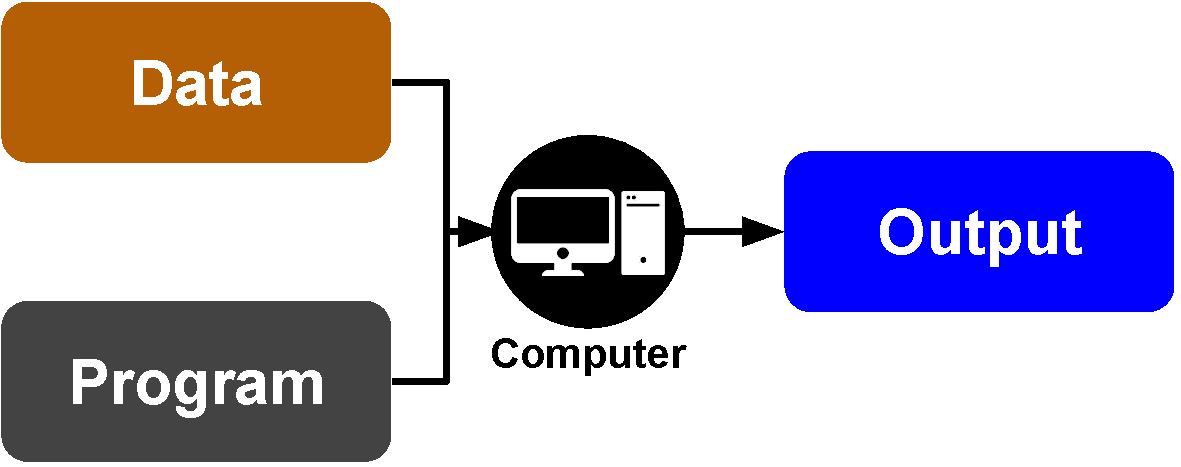
\includegraphics[width=\currprop]{figures/3_theoretical_background/shallow_learning/traditional_programming_pipeline.pdf} % + 0.19
    \caption{}
    \label{fig:traditional_programming_pipeline}
  \end{subfigure}
  \hfil % This provides the horizontal space
  \begin{subfigure}[c]{0.48\columnwidth} % Reduced width
    \centering
    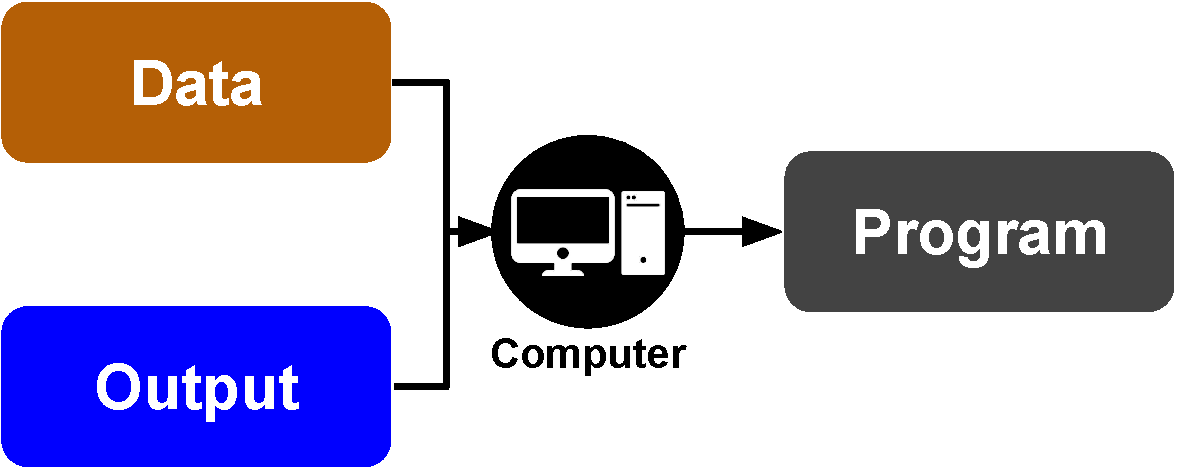
\includegraphics[clip,width=\currprop]{figures/3_theoretical_background/shallow_learning/machine_learning_pipeline.pdf}
    \caption{}
    \label{fig:machine_learning_pipeline}
  \end{subfigure}

  \fignote{(a) shows Classical Programming paradigm, while (b) shows the new Machine Learning paradigm.}
\end{figure}

\subsection{Shallow Learning models}

In this context, \ac{SL} is a \ac{ML} approach that works well for tabular data, but requires preprocessing steps for unstructured data (such as images, videos, texts, or \ac{SITS}) converting them into tabular data, a complete subfield called Feature Engineering \cite{zheng2018feature}. In addition to the requirement for handcrafted features, such models are generally older and less complex compared to current models, and the name ``shallow'' contrasts with \ac{DL}, which will be explained in more detail in Section \ref{sec:deep_learning}. Also, \ac{SL} models often require less data for training and are faster to train and implement, as well as being more interpretable, which makes it easier to understand how decisions are made by the model. However, to use them, it is necessary to choose those handcrafted features (extraction and selection), which can be challenging, especially in areas such as \ac{CV} and \ac{RS}.

\subsubsection{K-Nearest Neighbor (KNN)}

\acf{KNN} is an \ac{SL} classification model based on the principle that similar instances in a dataset tend to be located close to each other in the feature space space \citep{cover1967nearest}. Unlike other models that construct an explicit mathematical function during training, \ac{KNN} is classified as a lazy learner, as it does not generate a discriminative model in advance; instead, it stores the entire training dataset and postpones computational processing until the moment of inference. 

The algorithm's operation is based on calculating the distance between the sample to be classified and all examples in the training set -- usually the Euclidean distance, although other metrics such as Manhattan or Minkowski can be applied. The model selects the $K$ closest neighbors and defines the class of the new object by majority vote (see Figure \ref{fig:knn}). In the context of regression, \ac{KNN} estimates the output value using the arithmetic or weighted average of the values of the $K$ neighbors. However, its computational search cost increases linearly with the number of samples ($O(n)$) and is highly sensitive to the scale of the variables, requiring normalization steps and, often, dimensionality reduction techniques (such as PCA).

\begin{figure}[ht!]
    \centering
    \caption{Diagram of a K-nearest neighbor model.}
    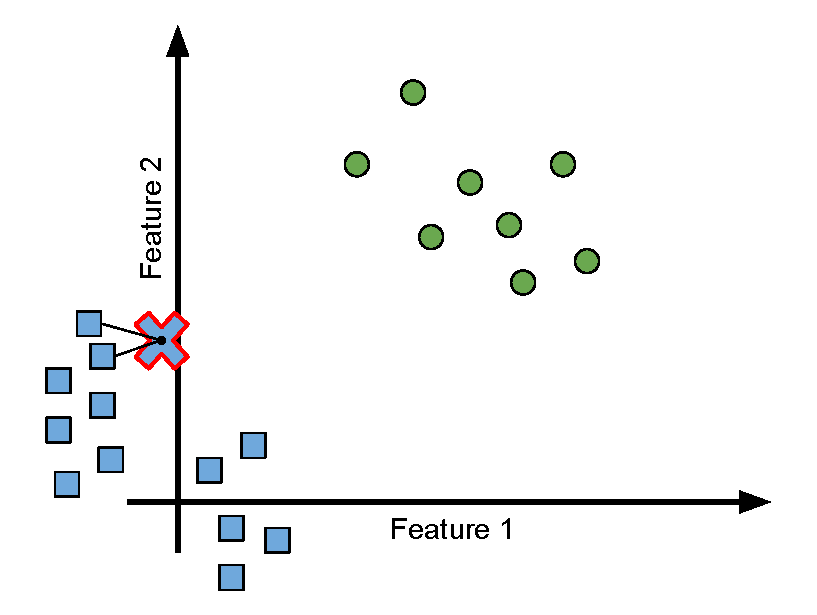
\includegraphics[width=.7\linewidth]{figures/3_theoretical_background/shallow_learning/knn.pdf}
    \fignote{One should notice that, in this model K=2 so, when a prediction sample is given (the X in the figure), the two most near training samples classes are verified, than their class will be assigned to the given prediction sample.}
    \label{fig:knn}
\end{figure}

\Ac{KNN} is widely used as a test for \ac{SSL} pre-training due to its simplicity and ability to provide a quick assessment of the quality of the generated embeddings, being retrained at each new pre-training epoch.

\subsubsection{Support Vector Machine (SVM)}

\Acf{SVM} is a widely used supervised learning algorithm for classification and regression tasks \citep{boser1992training}. SVM works by finding the optimal hyperplane that separates different classes of data in feature space, maximizing the margin between classes (see the Figure \ref{fig:svm}). In cases where the data is not linearly separable (such as spectral bands in \ac{RS}), \ac{SVM} can use the ``kernel trick'' to transform the data into a higher-dimensional space where linear separation is possible. \ac{SVM} is known for its effectiveness on high-dimensional datasets and its robustness against overfitting, especially when configured with the correct parameters.

\begin{figure}[ht!]
    \centering
    \caption{Diagram of a Support Vector Machine model.}
    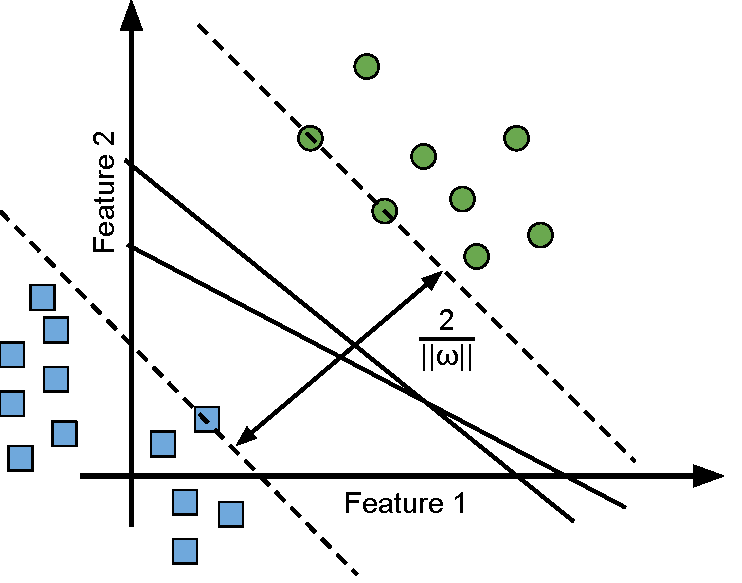
\includegraphics[width=.7\linewidth]{figures/3_theoretical_background/shallow_learning/svm.pdf}
    \label{fig:svm}
\end{figure}

The main idea behind the kernel trick is to map the input data to a higher-dimensional space where linear separation between classes can be achieved. Instead of explicitly calculating the coordinates of the data in this higher-dimensional space, the kernel trick allows us to directly calculate the inner products between the data vectors in the original space using specific kernel functions. The most common kernels include the Linear Kernel (for data that is already linearly separable), the Polynomial Kernel (which introduces curvature), and, notably, the Radial Basis Function (RBF) Kernel, which is one of the most widely used due to its effectiveness in dealing with complex separations in \ac{RS}.

Despite its theoretical robustness and good performance on many datasets, \ac{SVM} presents some practical challenges. First, the high computational cost and training time can be significant, especially with increasing data volume (very large datasets, such as pixels of multiespectral satellite images). Training time generally scales between $O(n^2)$ and $O(n^3)$ (where $n$ is the number of training samples), making it less efficient for large volumes of raw data than, for example, \ac{RF}. Second, \ac{SVM} performance is highly sensitive to the choice and adjustment of Kernel parameters (hyperparameters) and the penalty parameter ($C$). As such, \ac{SVM} usually requires several different long training sessions (with different hyperparameters), making the model quite costly.

\subsubsection{Random Forest (RF)}
\label{sec:rf}

\Acf{RF} is a \ac{SL} model that combines multiple simpler models, \acf{DT}, to improve the quality and robustness of predictions \citep{breiman2001random}. A \ac{DT} (see the black bounding box in Figure \ref{fig:random_forest}) works by recursively dividing a dataset into smaller, more homogeneous subsets based on input characteristics (variables) \citep{quinlan1986induction}. Although simple and interpretable, a single \ac{DT} is often susceptible to overfitting, which means that it may perform well on training data but poorly on test data. However, on the plus side, it is one of the most interpretable models in the entire field of machine learning, precisely because it approximates the way humans think about tasks or define classes, as exemplified above.

\begin{figure}[ht!]
    \centering
    \caption{Diagram of a Random Forest model.}
    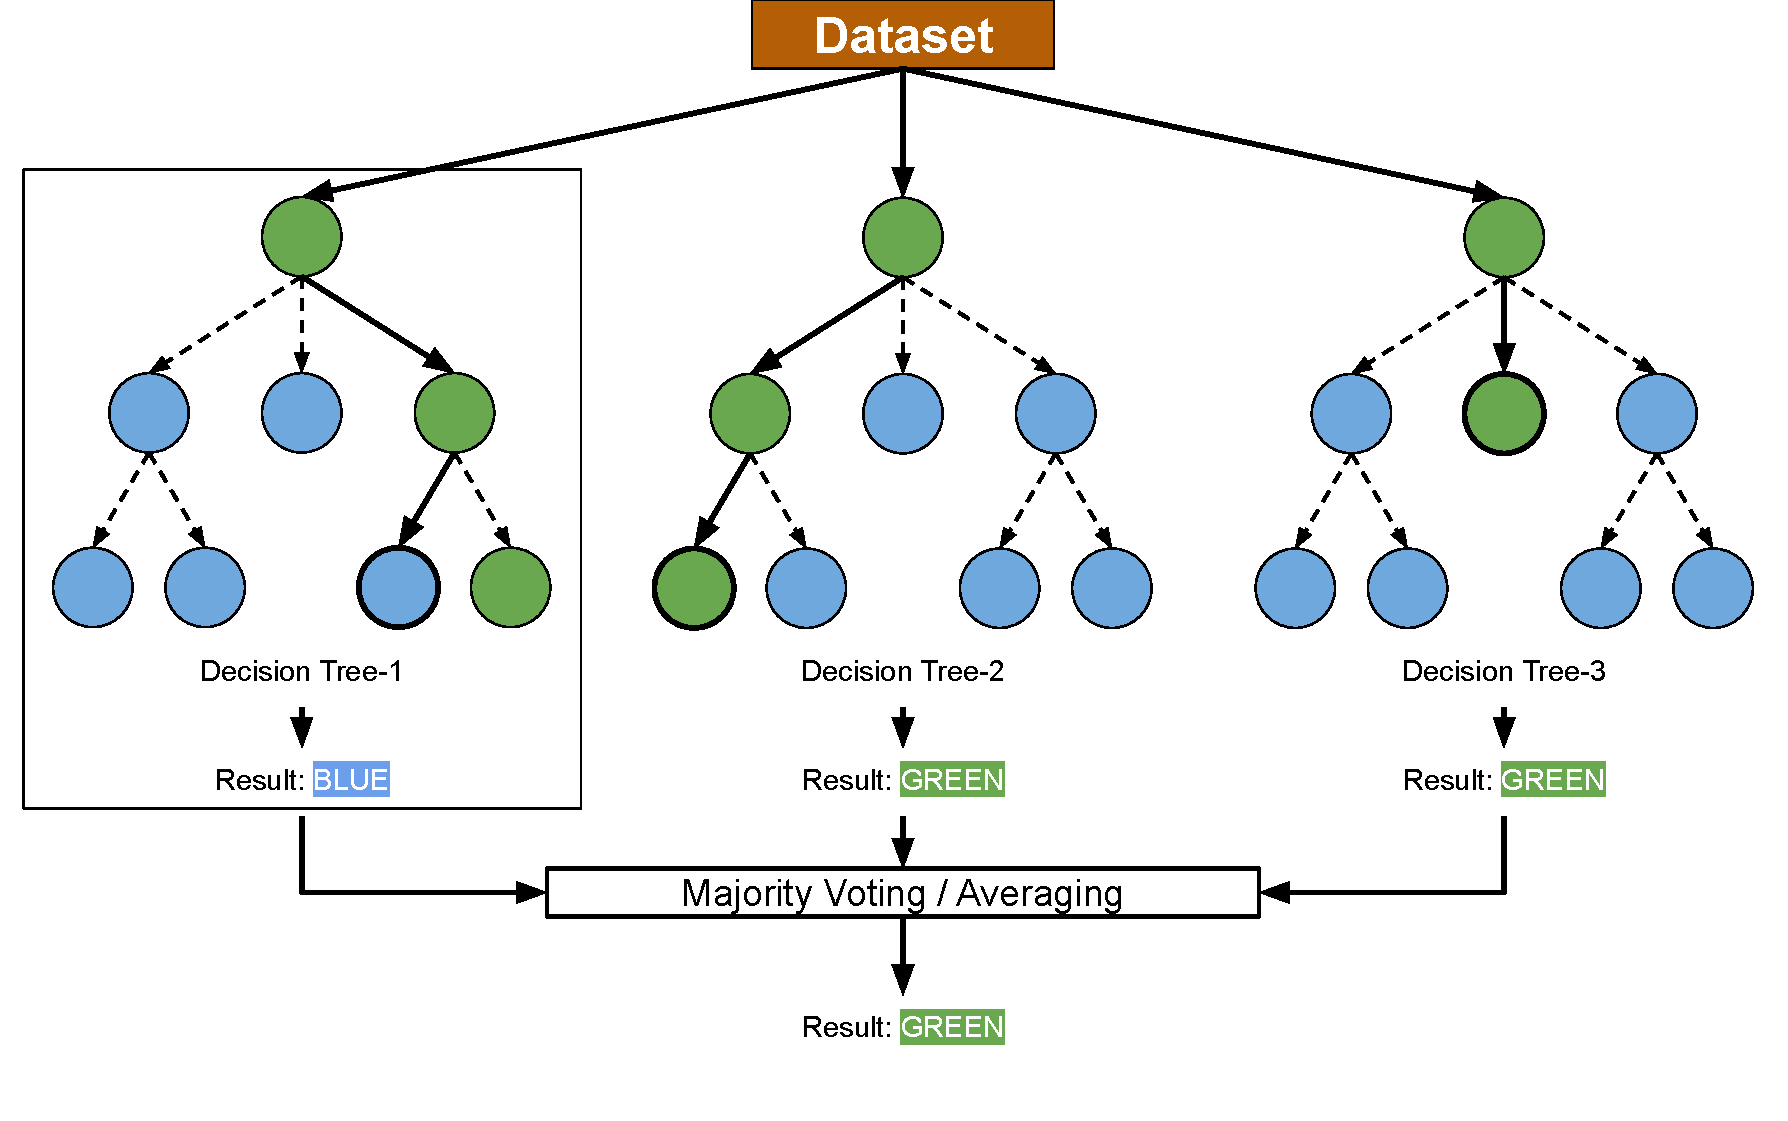
\includegraphics[width=1\linewidth]{figures/3_theoretical_background/shallow_learning/random_forest.pdf}
    \fignote{The black bounding box is highlighting a decision tree, the core subpart of a RF.}
    \label{fig:random_forest}
\end{figure}

In \ac{RS}, \ac{RF} is a classification tool that is still widely used today, mainly for \ac{LULC}. It is widely used because it does not require data preprocessing, being one of the few models that is robust to data scale. Thus, it is quite common to classify image pixels or satellite mosaics, creating thematic maps in shallow semantic segmentation. Due to its training speed and lack of preprocessing requirements, it is also a widely used model as a baseline for more advanced techniques.

\subsubsection{Gradient Boosting (GB)}

\Acf{GB} models, on the other hand, are very similar to \ac{RF} (see Section \ref{sec:rf}), as they also build multiple \ac{DT} to improve predictive performance \citep{friedman2001greedy}. However, while \ac{RF} builds trees independently and joins them together, \ac{GB} builds trees sequentially, where each new tree attempts to correct the errors of the previous trees. This process is known as boosting, and the goal is to minimize a specific loss function by iteratively adding weak models that improve the overall performance of the model.

\begin{figure}[ht!]
    \centering
    \caption{Diagram of a Gradient Boosting (GB) model.}
    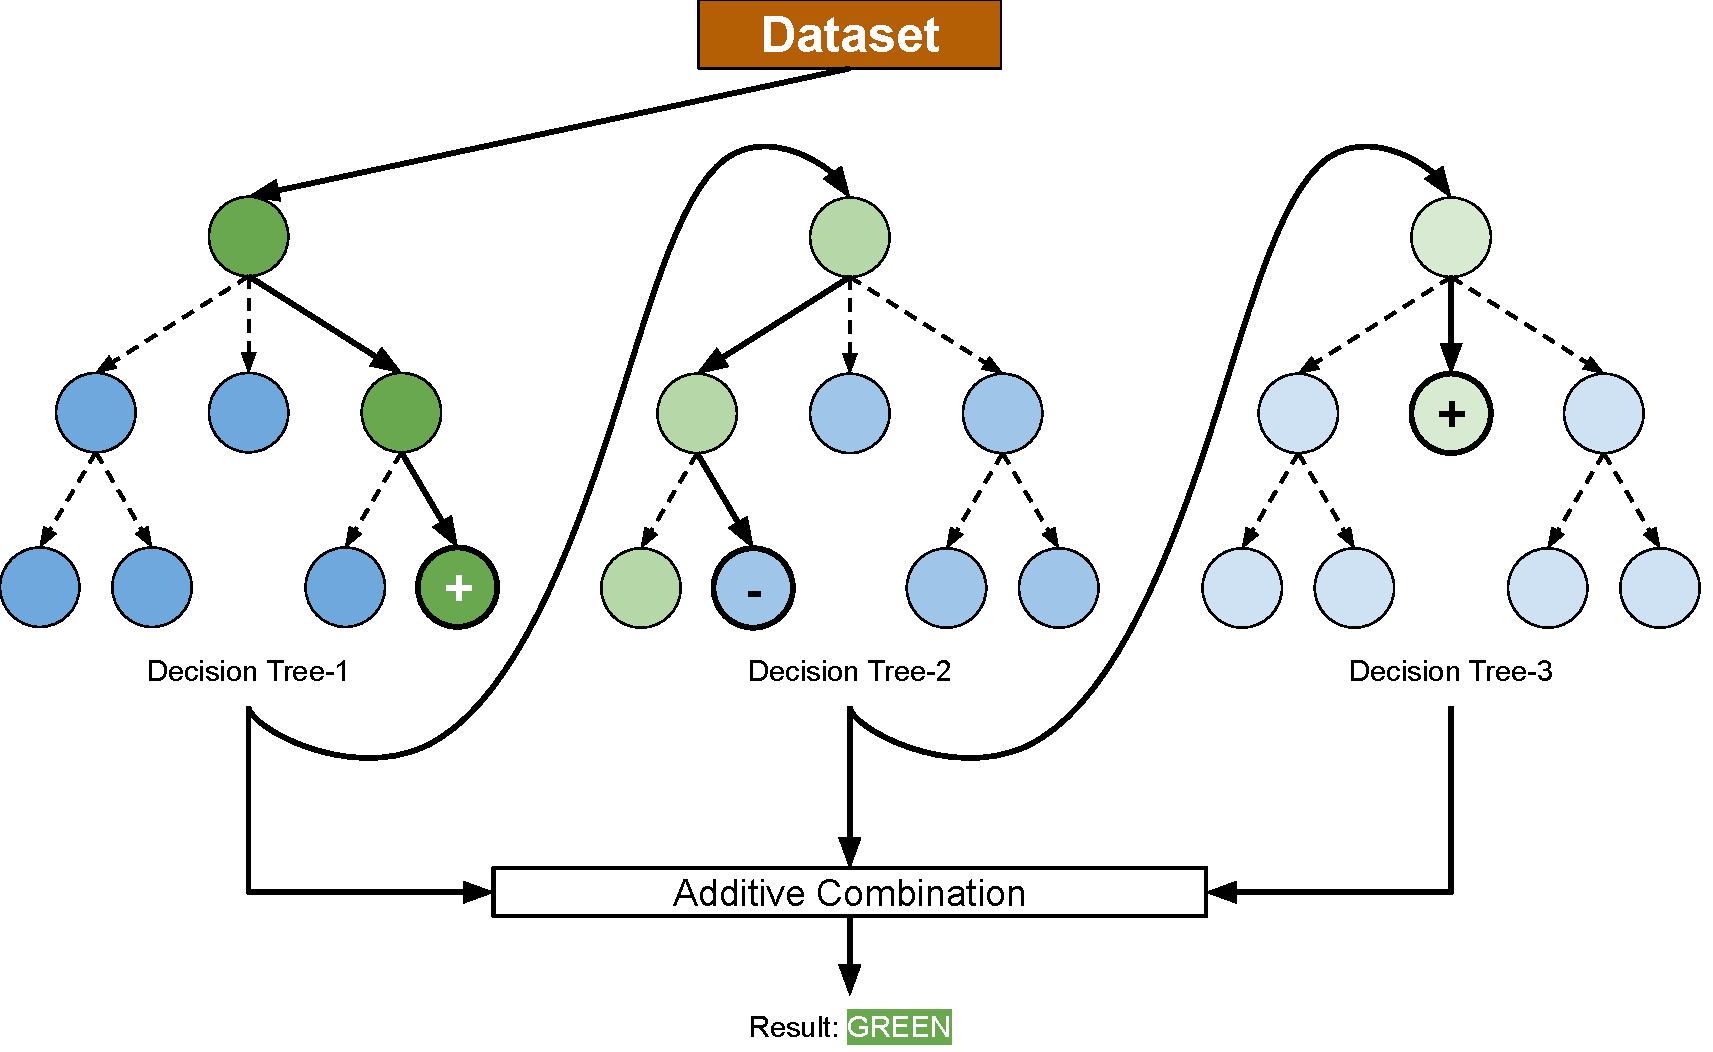
\includegraphics[width=1\linewidth]{figures/3_theoretical_background/shallow_learning/gradient_boosting.pdf}
    \fignote{One should notice that the Decision Trees refine each other's decisions.}
    \label{fig:gradient_boosting}
\end{figure}

In \ac{RS}, \ac{GB} has uses that are extremely similar to RF, functioning as a more costly
alternative - both in terms of computational cost and scientist time - but ofter with better results. Two famous implementations of \ac{GB} stand out: XGBoost and LightGBM. The main difference in standard hyperparameter optimization strategies between LightGBM and XGBoost lies in the treatment of the tree: LightGBM uses depth-based (leaf-wise) tree growth, generally resulting in deeper and more asymmetric \ac{DT} by default, while XGBoost typically uses level-wise growth, producing balanced \ac{DT}, which directly affects the standard parameters of maximum depth and number of leaves, both of which are widely used in \ac{RS}.

\subsubsection{Multi-Layer Perceptron (MLP)}
\label{sec:mlp}

The \ac{MLP} is a classic Artificial Neural Network (ANN) architecture consisting of multiple layers of fully connected neurons, i.e., each neuron in one layer is connected to all neurons in the next layer \citep{rosenblatt1958perceptron, rumelhart1986learning}. Such a model is also called a Feedforward Neural Network (FNN). The \ac{MLP} is composed of an input layer, one or more hidden layers, and an output layer. The hidden layers apply nonlinear activation functions, such as \ac{ReLU} or sigmoid, to introduce nonlinearity to the model.

\begin{figure}[ht!]
    \centering
    \caption{Diagram of a Multi-Layer Perceptron.}
    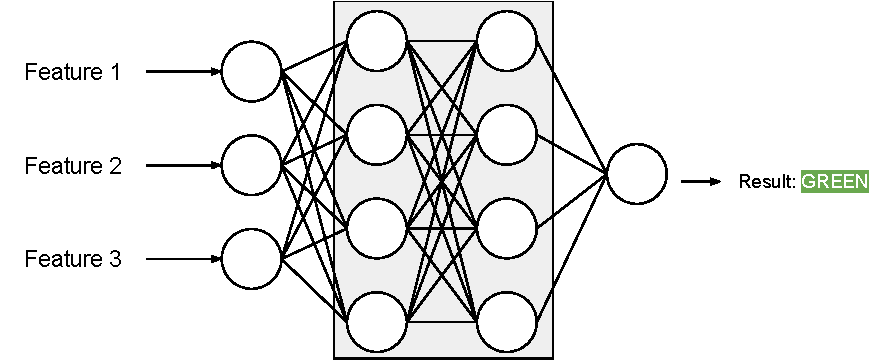
\includegraphics[width=.8\linewidth]{figures/3_theoretical_background/deep learning/mlp.pdf}
    \label{fig:mlp}
\end{figure}

Historically, \ac{MLP} represents the foundational architecture for \ac{DL} models. While deep configurations exist, simpler implementations with few hidden layers are often categorized alongside shallow methods. Today, \acs{MLP}s are still used at the end of other more complex neural networks to perform the final step of mapping the extracted features to the desired classes or output values. Also, this model is often used as baselines.

\subsubsection{K-Means}

K-Means is possibly the best known and most widely used Unsupervised \ac{SL} model \citep{macqueen1965some, lloyd1982least}. Unsupervised Learning is a \ac{ML} technique where the model is trained using an unlabeled dataset, i.e., the input examples do not have associated desired outputs. The goal of the model is to identify patterns, structures, or clusters in the data without the guidance of predefined labels. K-Means is a clustering algorithm that aims to partition a data set into K distinct groups, where each group is represented by a centroid. The algorithm works iteratively, assigning each data point to the nearest centroid and then recalculating the centroids based on the new assignments. This process continues until the assignments of the data points no longer change significantly or until a maximum number of iterations is reached.

\begin{figure}[ht!]
    \centering
    \caption{The impact of applying K-Means in a Unlabeled Dataset.}
    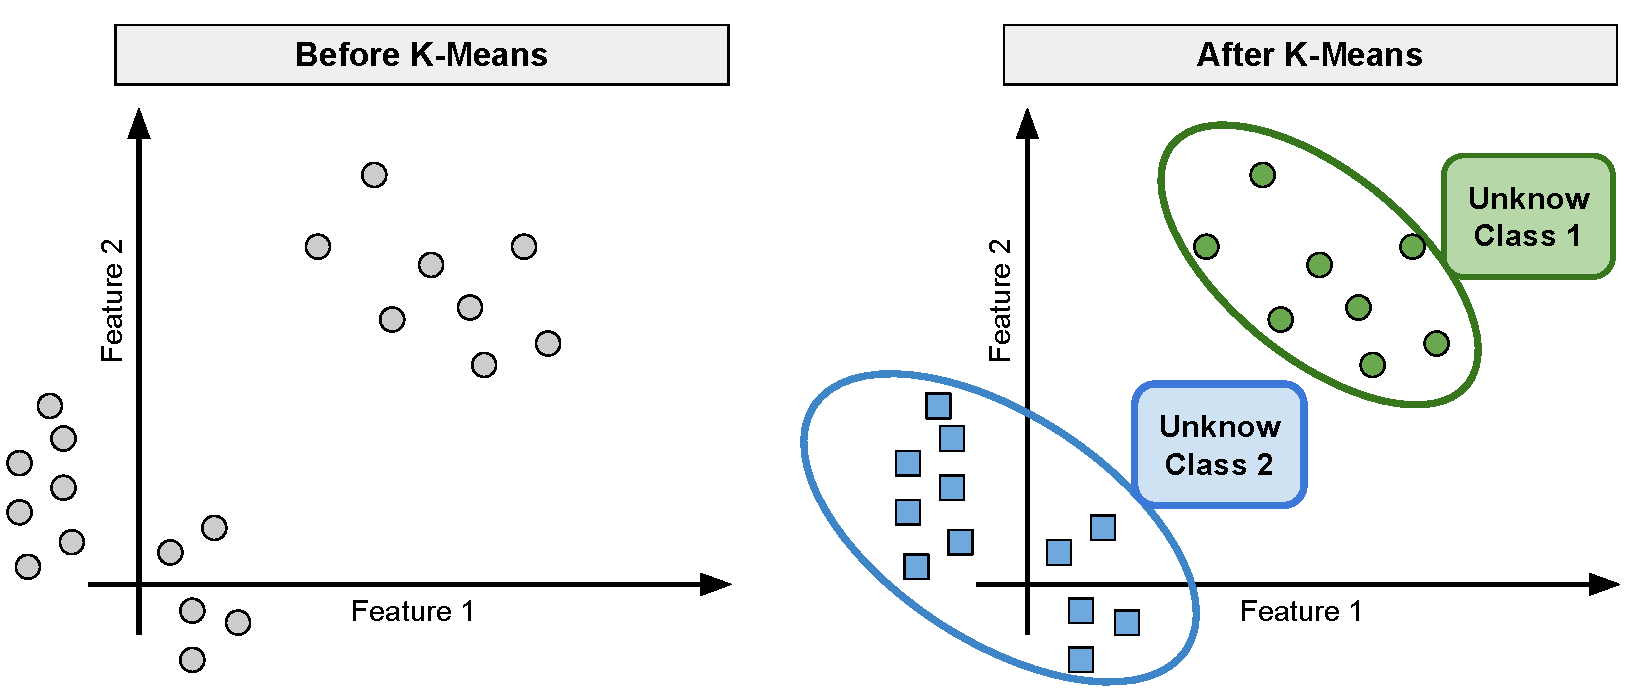
\includegraphics[width=1\linewidth]{figures/3_theoretical_background/shallow_learning/kmeans.pdf}
    \label{fig:kmeans}
\end{figure}

The big challenge is to define the value of $K$, which can be done using methods such as the elbow method or silhouette score. In \ac{RS}, K-Means is often used for image segmentation, where the goal is to group pixels with similar spectral characteristics, facilitating the identification of different types of \ac{LULC}, serving both to facilitate exploratory analysis and to assist in subsequent supervised classification tasks.

\subsubsection{Gaussian Mixture Model (GMM)}

The \acf{GMM} is an \ac{SL} unsupervised model that assumes that all data points are generated from a mixture of a finite number of Gaussian distributions with unknown parameters \citep{dempster1977maximum}. While K-Means performs hard clustering, where each point belongs exclusively to a centroid/cluster, \ac{GMM} performs soft clustering, in which the model provides the probability of a given data point belonging to each of the clusters, allowing for a more robust handling of uncertainties and class overlaps.

The model is adjusted using the Expectation-Maximization (EM) algorithm. In the Expectation step, the algorithm estimates the probability of each point belonging to each Gaussian component; in the Maximization step, the Gaussian parameters (mean, covariance, and mixture weight) are updated to maximize the likelihood of the observed data. Also similar to K-Means, to use \ac{GMM} it is necessary to determine the number of components (clusters) to be used (see Figure \ref{fig:gmm}).

\begin{figure}[ht!]
    \centering
    \caption{Diagram of a Gaussian Mixture Model.}
    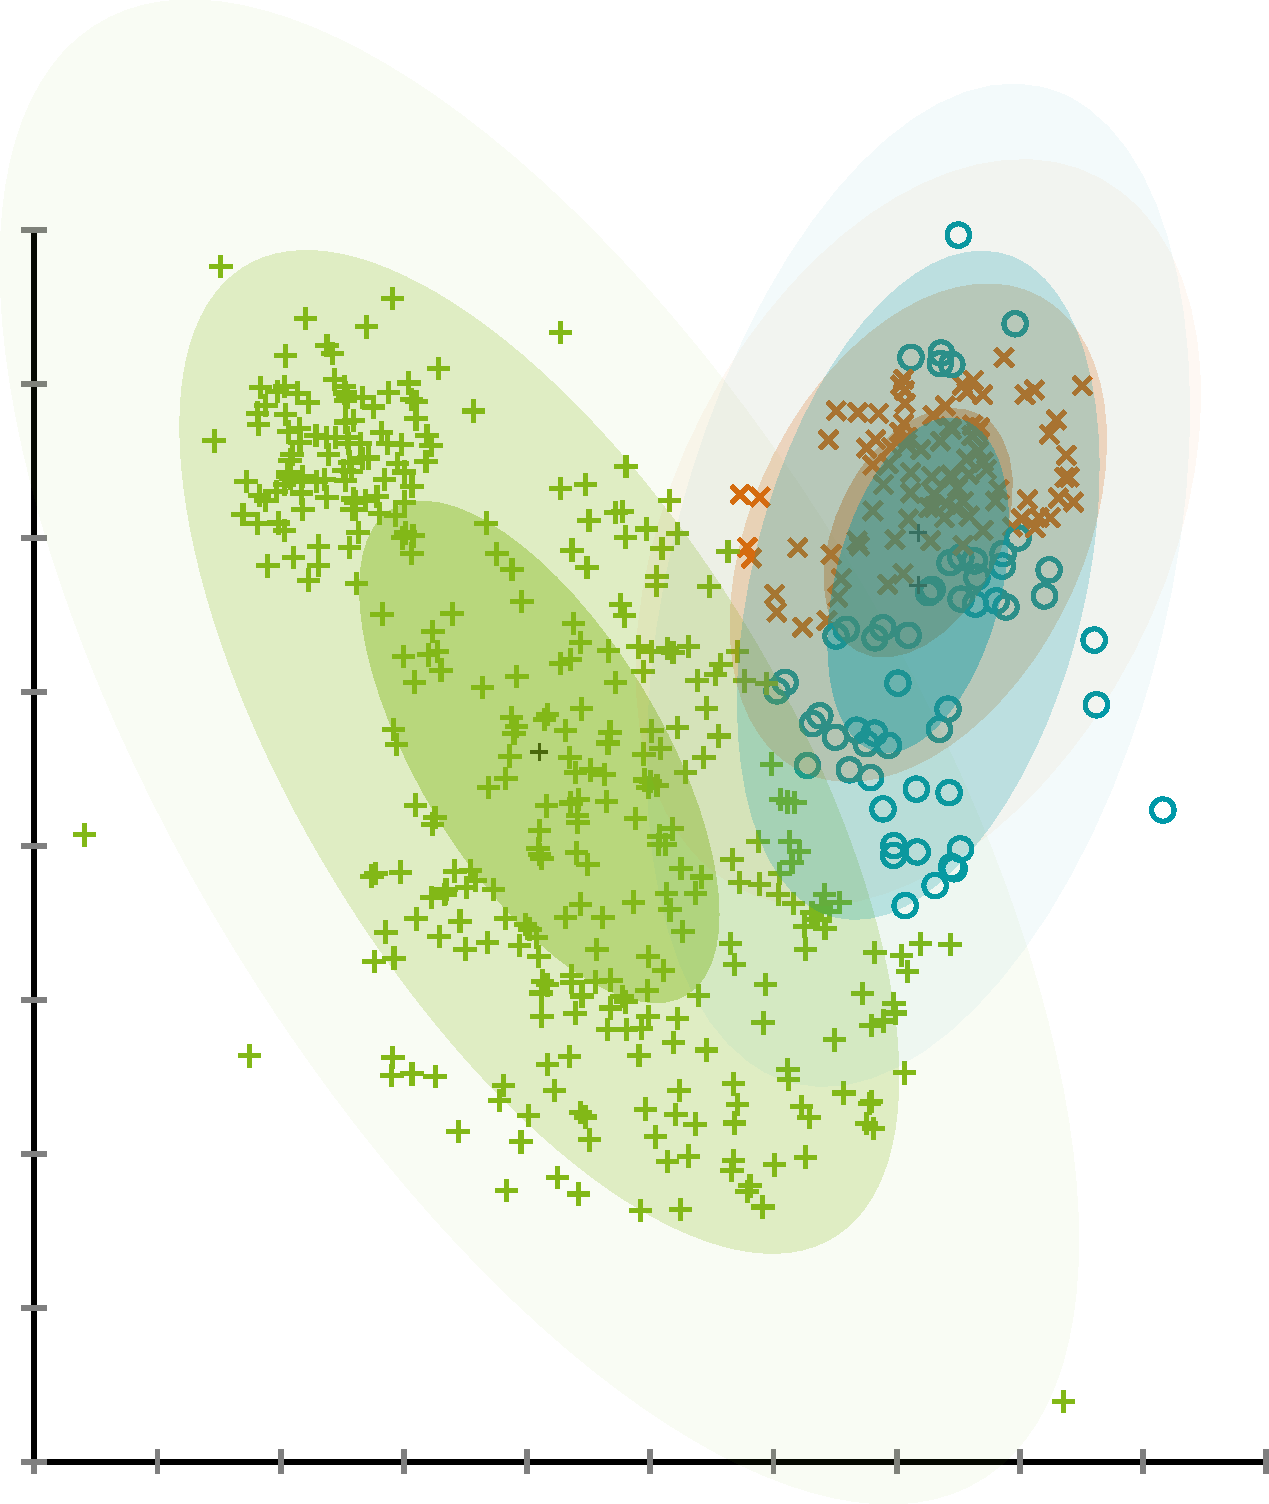
\includegraphics[width=.7\linewidth]{figures/3_theoretical_background/shallow_learning/gmm.pdf}
    \fignote{This example shows a GMM with number of components=3. Adapted from \href{https://dm.cs.tu-dortmund.de/mlbits/cluster-em-gmm-demo/}{TU Dortmund}}
    \label{fig:gmm}
\end{figure}


\subsection{Deep Learning models}
\label{sec:deep_learning}

On the other hand, \ac{DL} is a Machine Learning approach that uses latent data representations, meaning that the model itself learns to extract relevant features from raw data, eliminating the need for manual handcrafted feature extraction (with the exception, of course, of data normalization, which helps in model training convergence) \cite{bishop2023deep}. The best-known \ac{DL} models are Artificial Neural Networks (ANNs), which are composed of multiple layers of interconnected artificial neurons \cite{goodfellow2016deep}. Each neuron receives inputs, applies an activation function, and transmits the output to the neurons in the next layer. A loss function is defined to quantify the difference between the model's predictions and the actual values, and the model is trained using optimization algorithms, such as gradient descent, to adjust the weights of the connections between neurons in order to minimize this loss. In supervised learning, the most common loss functions include cross-entropy for classification and mean squared error for regression, which directly compare the model's predictions with the actual labels during training. Unsupervised techniques is also used in \ac{DL} to learn representations of data without explicit labels with different loss functions.

\subsubsection{Convolutional Neural Network (CNN)}
\label{sec:cnn}

A \ac{CNN} is a \ac{DL} model specially designed to process images \citep{lecun1989backpropagation}. \ac{CNN} are composed of convolutional layers that apply filters (or kernels) to extract local features from the input data, such as edges, textures, and spatial patterns. These layers are followed by pooling layers, which reduce the dimensionality of the data while retaining the most important features. Finally, an \ac{MLP} (see Section \ref{sec:mlp}) is generally used to perform classification or regression based on the extracted features.

\begin{figure}[ht!]
    \centering
    \caption{Diagram of a Convolutional Neural Network.}
    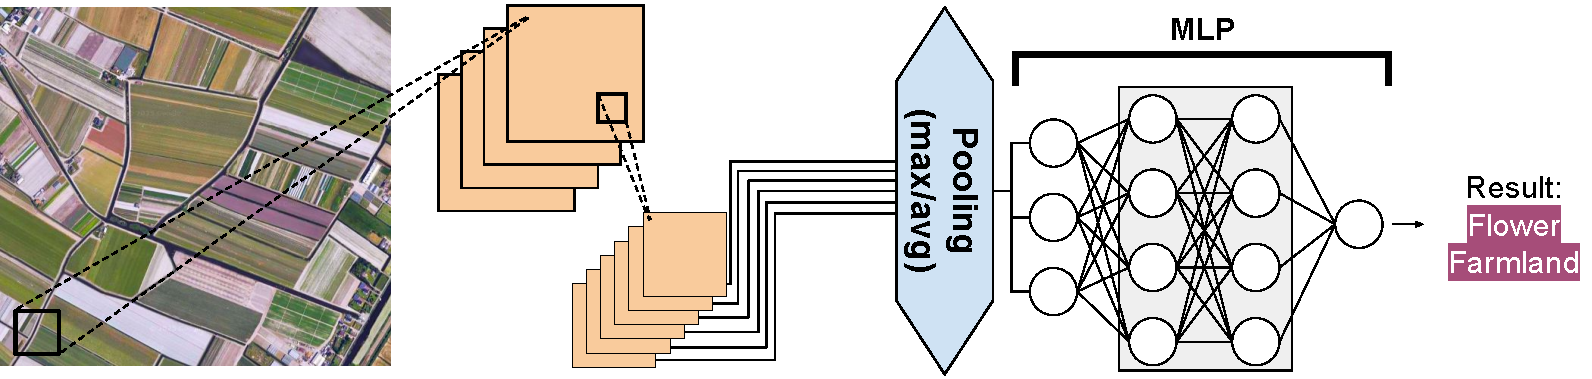
\includegraphics[width=1\linewidth]{figures/3_theoretical_background/deep learning/cnn.pdf}
    \label{fig:cnn}
\end{figure}

The motivation behind \ac{CNN} is to avoid the extremely high number of parameters that an \ac{MLP} would have when dealing with images, which generally have high dimensionality. For example, a $256\times256$ pixel Sentinel 2 image has $655360$ entries ($256 \times 256 \times 10$), which would result in millions of parameters in a typical \ac{MLP}. \acs{CNN}s allow kernels- such as Sobel and Canny kernels- to be trained and customized for each dataset, drastically reducing the number of parameters and making training possible.

The history of \acp{CNN} began with its use for character recognition \citep{lecun1989backpropagation} and the consolidation of LeNet-5 \citep{lecun2002gradient}, but it was AlexNet \citep{krizhevsky2012imagenet} that revolutionized the field by demonstrating the potential of GPUs -- which led to their widespread use throughout the field of machine learning -- and the \ac{ReLU} function in deep networks. This was followed by approaches such as VGG \citep{simonyan2014very}, focused on depth with small filters, and GoogleNet \citep{szegedy2015going}, which introduced Inception modules for multiscale processing, a technique refined in subsequent versions \citep{szegedy2016rethinking,szegedy2017inception}. A definitive milestone was ResNet \citep{he2016deep}, whose residual connections that dealt with Vanishing Gradients enabled networks with hundreds of layers, underpinning models such as ResNeXt \citep{xie2017aggregated}, based on cardinality, and DenseNet \citep{huang2017densely}, which prioritizes feature reuse (see Figure \ref{fig:cnn_hist}).

\begin{figure}[ht!]
    \centering
    \caption{Historical diagram of the evolution of Convolutional Neural Networs.}
    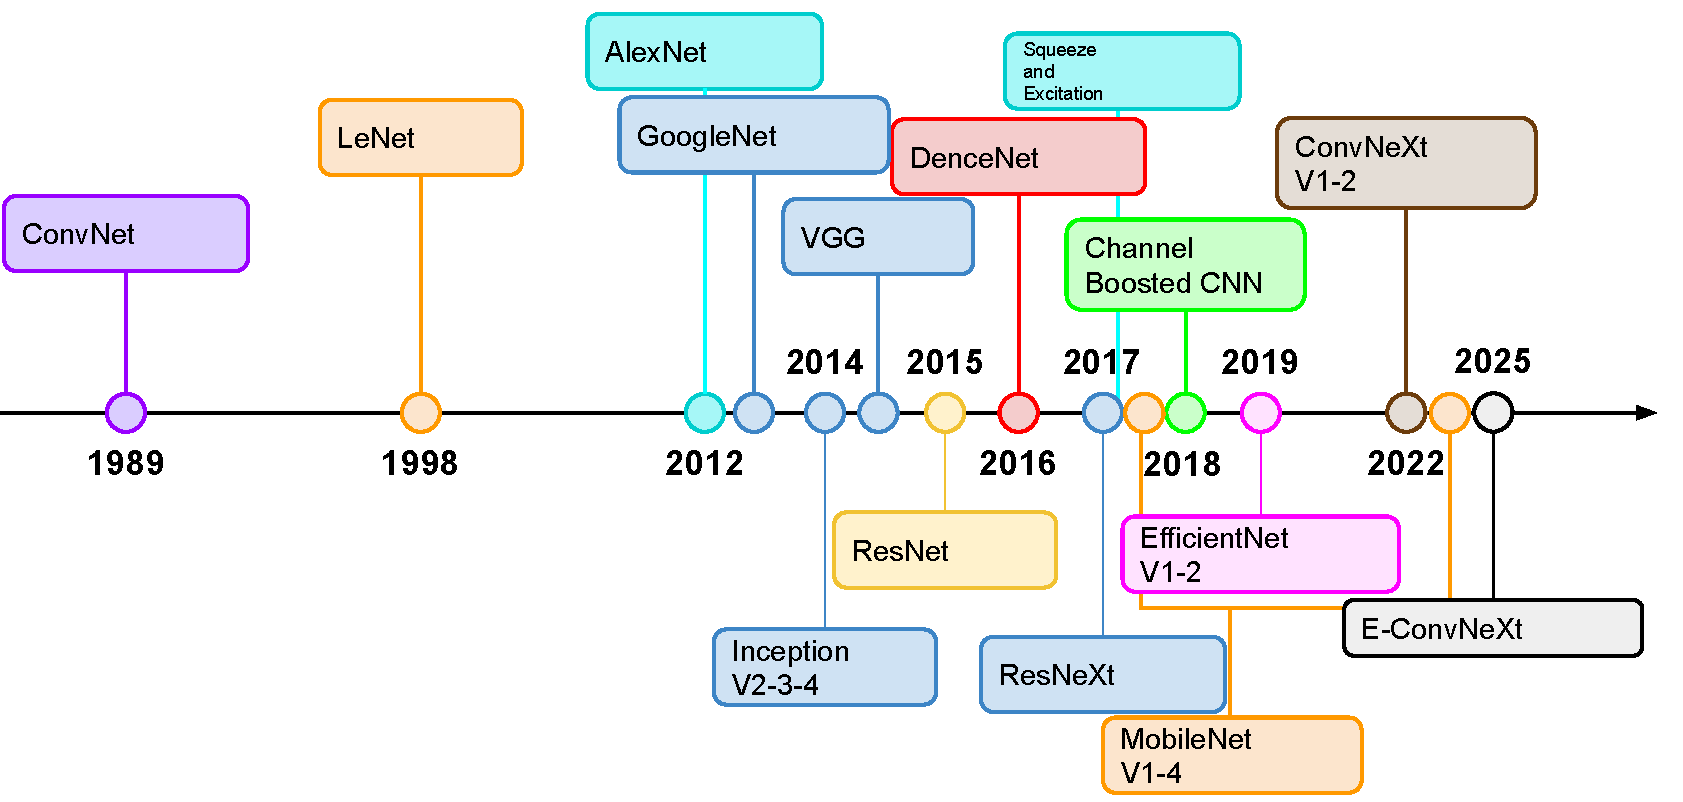
\includegraphics[width=1\linewidth]{figures/3_theoretical_background/deep learning/cnn_history.pdf}
    \label{fig:cnn_hist}
\end{figure}

Recently, efficiency has become the priority with the EfficientNet family \citep{tan2019efficientnet,tan2021efficientnetv2}, which optimized the width and depth scaling of networks. Being contemporary, the MobileNet series \citep{howard2017mobilenetsefficientconvolutionalneural,sandler2019mobilenetv2invertedresidualslinear,howard2019searchingmobilenetv3,qin2024mobilenetv4universalmodels} leveraged depthwise separable convolutions to balance latency and accuracy in resource-constrained environments. Concurrently, Squeeze-and-Excitation networks \citep{hu2019squeezeandexcitationnetworks} introduced channel-wise attention mechanisms to explicitly model interdependencies between channels, enhancing representational power with minimal computational overhead. In response to the rise of Transformers, the ConvNeXt architecture \citep{liu2022convnet} modernized \acp{CNN} with contemporary design choices, evolving to V2 \citep{woo2023convnext} with the use of masked autoencoders and to E-ConvNeXt \citep{wang2025convnext}, focused on low-resource devices. Complementarily, approaches such as Channel Boosted CNN \citep{khan2018new} explored channel diversity via transfer learning in an attempt to keep \acp{CNN} competitive in the face of new computer vision paradigms, especially in scenarios with low computational resources or little data.

\subsubsection{Semantic Segmentation Models}
\label{sec:fcn}

Some adaptions were done to convert \ac{CNN}s (see Section \ref{sec:cnn}) for semantic segmentation tasks, where the goal is to classify each pixel in an image into a specific class. One of the first adaptations, and still widely used today, is the \acf{FCN} \citep{long2015fully}. The strategy used was to replace the typical final \ac{MLP} of \ac{CNN} with deconvolution (or upsampling) layers, allowing the network to process images of any size and produce corresponding segmentation maps (see Figure \ref{fig:fcn}) .

\begin{figure}[ht!]
    \centering
    \caption{Diagram of a Fully Convolutional Network model.}
    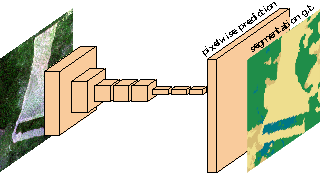
\includegraphics[width=.75\linewidth]{figures/3_theoretical_background/deep learning/fcn.pdf}
    \fignote{Adapted from Long et al \citep{long2015fullyconvolutionalnetworkssemantic}}
    \label{fig:fcn}
\end{figure}

This architecture is especially useful in \ac{RS} for LULC and Parcel Delineation applications -- as they are intrinsically semantic segmentation applications -- in addition to some uses in Crop Mapping or Crop Yielding. Furthermore, variations in which two \ac{FCN} are combined and have their embeddings concatenated are also used for Change Detection.

Aside from the FCN strategy, another common strategy for semantic segmentation networks is that of encoder-decoder networks, such as the U-Net model. U-Net was designed for biomedical image segmentation tasks, but is also possibly the most historically used \ac{DL} model in \ac{RS} \citep{ronneberger2015u}. The main innovation of U-Net is its ``U''-shaped structure, which consists of a path of reduced spatial resolution and increased number of channels (encoder) and subsequently a path of increased spatial resolution and decreased number of channels (decoder). The encoder follows a design pattern similar to that of \ac{CNN}, using blocks containing convolutional layers, \ac{ReLU} activation, and max pooling. On the other hand, the decoder is composed of upsampling and convolution layers, which help to reconstruct the spatial resolution of the image. This architecture allows the network to capture contexts of different scales while maintaining accurate spatial information. The Decision Factor of U-Net is the skip connections that link the corresponding layers of the encoder and decoder, allowing detailed information to be transferred directly to the reconstruction process, significantly improving segmentation accuracy (see Figure \ref{fig:unet}).

\begin{figure}[ht!]
    \centering
    \caption{Diagram of a U-Net model.}
    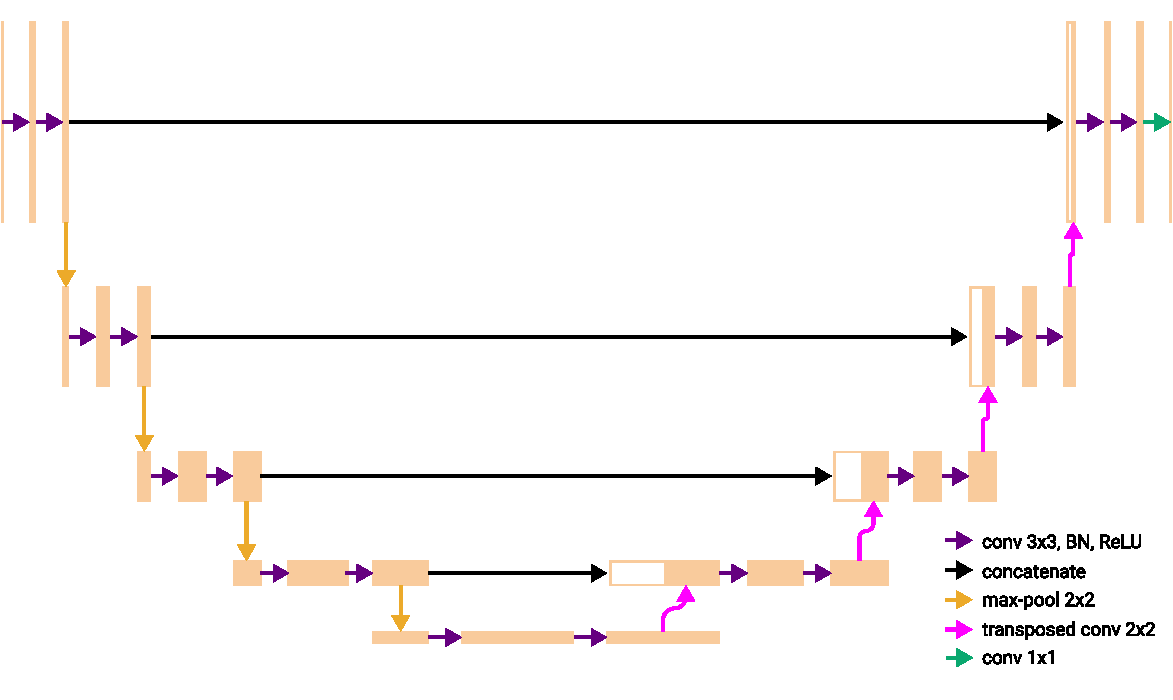
\includegraphics[width=0.8\linewidth]{figures/3_theoretical_background/deep learning/unet.pdf}
    \fignote{One should notice that the model layers ressemble a U. Adapted from \href{https://innolitics.com/articles/medical-image-segmentation-overview/}{Innolitics}}
    \label{fig:unet}
\end{figure}

Several variations of U-Net have been proposed over the years, such as U-Net++ and Attention U-Net, which introduce improvements in skip connections to increase the accuracy and efficiency of the model. In addition, there are also variations that change the encoder to classics \acs{CNN}s architectures such as ResNet or EfficientNet - without using the final \ac{MLP} (see Section \ref{sec:mlp}) - aiming to improve the model's feature extraction capability.


\subsubsection{AutoEncoder (AE)}

\Acf{AE} is a \ac{DL} architecture designed to learn compressed representations of input data, usually for dimensionality reduction or feature learning later used in another model \citep{hinton2006reducing}. An autoencoder consists of two main parts: the encoder and the decoder. The encoder maps the input data to a lower-dimensional latent space, compressing the information, while the decoder reconstructs the original data from this compressed representation (see Figure \ref{fig:autoencoder}).

\begin{figure}[ht!]
    \centering
    \caption{Diagram of a AutoEncoder model.}
    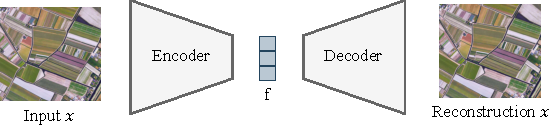
\includegraphics[width=0.85\linewidth]{figures/3_theoretical_background/deep learning/autoencoder.pdf}
    \fignote{Adapted from \href{https://uvadlc-notebooks.readthedocs.io/en/latest/tutorial_notebooks/tutorial9/AE_CIFAR10.html}{UvA Deep Learning Tutorials}}
    \label{fig:autoencoder}
\end{figure}

There are several types of autoencoders, including Denoising Autoencoders, which learn to reconstruct noisy data, and Variational Autoencoders (VAEs), which introduce a probabilistic approach to data generation - allowing, for example, the generation of data that mixes different classes. In \ac{RS}, autoencoders are often used for pretraining models, but this topic will be better addressed in Section \ref{sec:ssl_contextualization}.

\subsubsection{Generative Adversarial Network (GAN)}

\Acf{GAN} is a DL architecture composed of two neural models that compete with each other: the generator and the discriminator. The generator creates synthetic data from a random input, while the discriminator attempts to distinguish between real and generated data. During training, both models are trained, the generator learns to create increasingly realistic data, while the discriminator becomes more effective at identifying false data (see Figure \ref{fig:gan}). The convergence of this process is theoretically guaranteed by the ``Nash equilibrium'', in which both the generator and the discriminator have no significant gains in changing their strategy, although this is usually only seen approximately in practice.

\begin{figure}[ht!]
    \centering
    \caption{Diagram of a Generative Adversarial Network model.}
    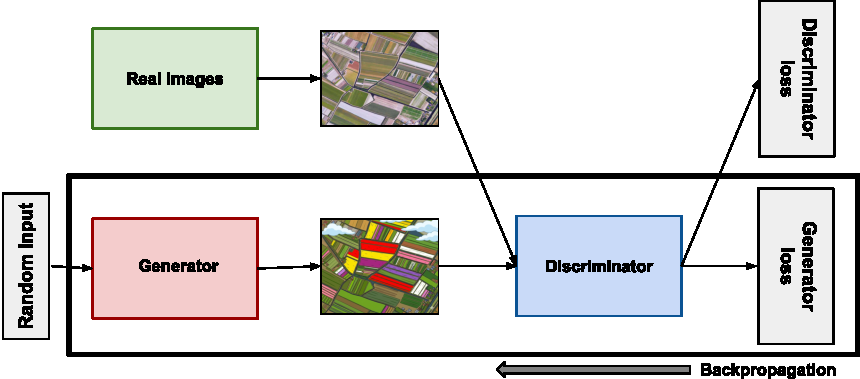
\includegraphics[width=1\linewidth]{figures/3_theoretical_background/deep learning/gan.pdf}
    \fignote{Adapted from \href{https://developers.google.com/machine-learning/gan/generator}{Google Developers}}
    \label{fig:gan}
\end{figure}

In \ac{RS}, \acs{GAN}s are used for various applications, such as synthetic image generation, image translation between different domains (e.g., from radar images to optical images), and especially for super-resolution of satellite images \citep{goodfellow2014generative}. In addition, \acs{GAN}s are also used to augment limited datasets by generating additional samples that help improve the performance of supervised models, which is useful for scenarios with very little data, as is often the case with Crop Yielding. However, \acs{GAN}s are known to potentially generate artifacts in the images they produce, which can be a challenge in applications that require high fidelity, in addition to the impossibility of auditing the generated data, making them difficult to use in applications such as deforestation Change Detection.


\subsubsection{Recurrent Neural Network (RNN)}
\label{sec:rnn}

A \ac{RNN} is a \ac{DL} model designed to handle sequential data, used in \ac{RS} for time series processing, whether pixels or images, through hybrid models with \ac{CNN}. \acs{RNN}s have recurrent connections that allow information from previous steps in the sequence to be retained and used to influence predictions in subsequent steps.

\acs{RNN}s work through a hidden state ($h_t$) that is updated at each step of the sequence ($x_t$), allowing the model to capture temporal dependencies in the data and produce an output ($y_t$) at each step (see Figure \ref{fig:rnn}). However, they suffer from the problem of gradient vanishing, which makes it difficult to learn long-term dependencies in long sequences.

\begin{figure}[ht!]
    \centering
    \caption{Diagram of a Recurrent Neural Network model.}
    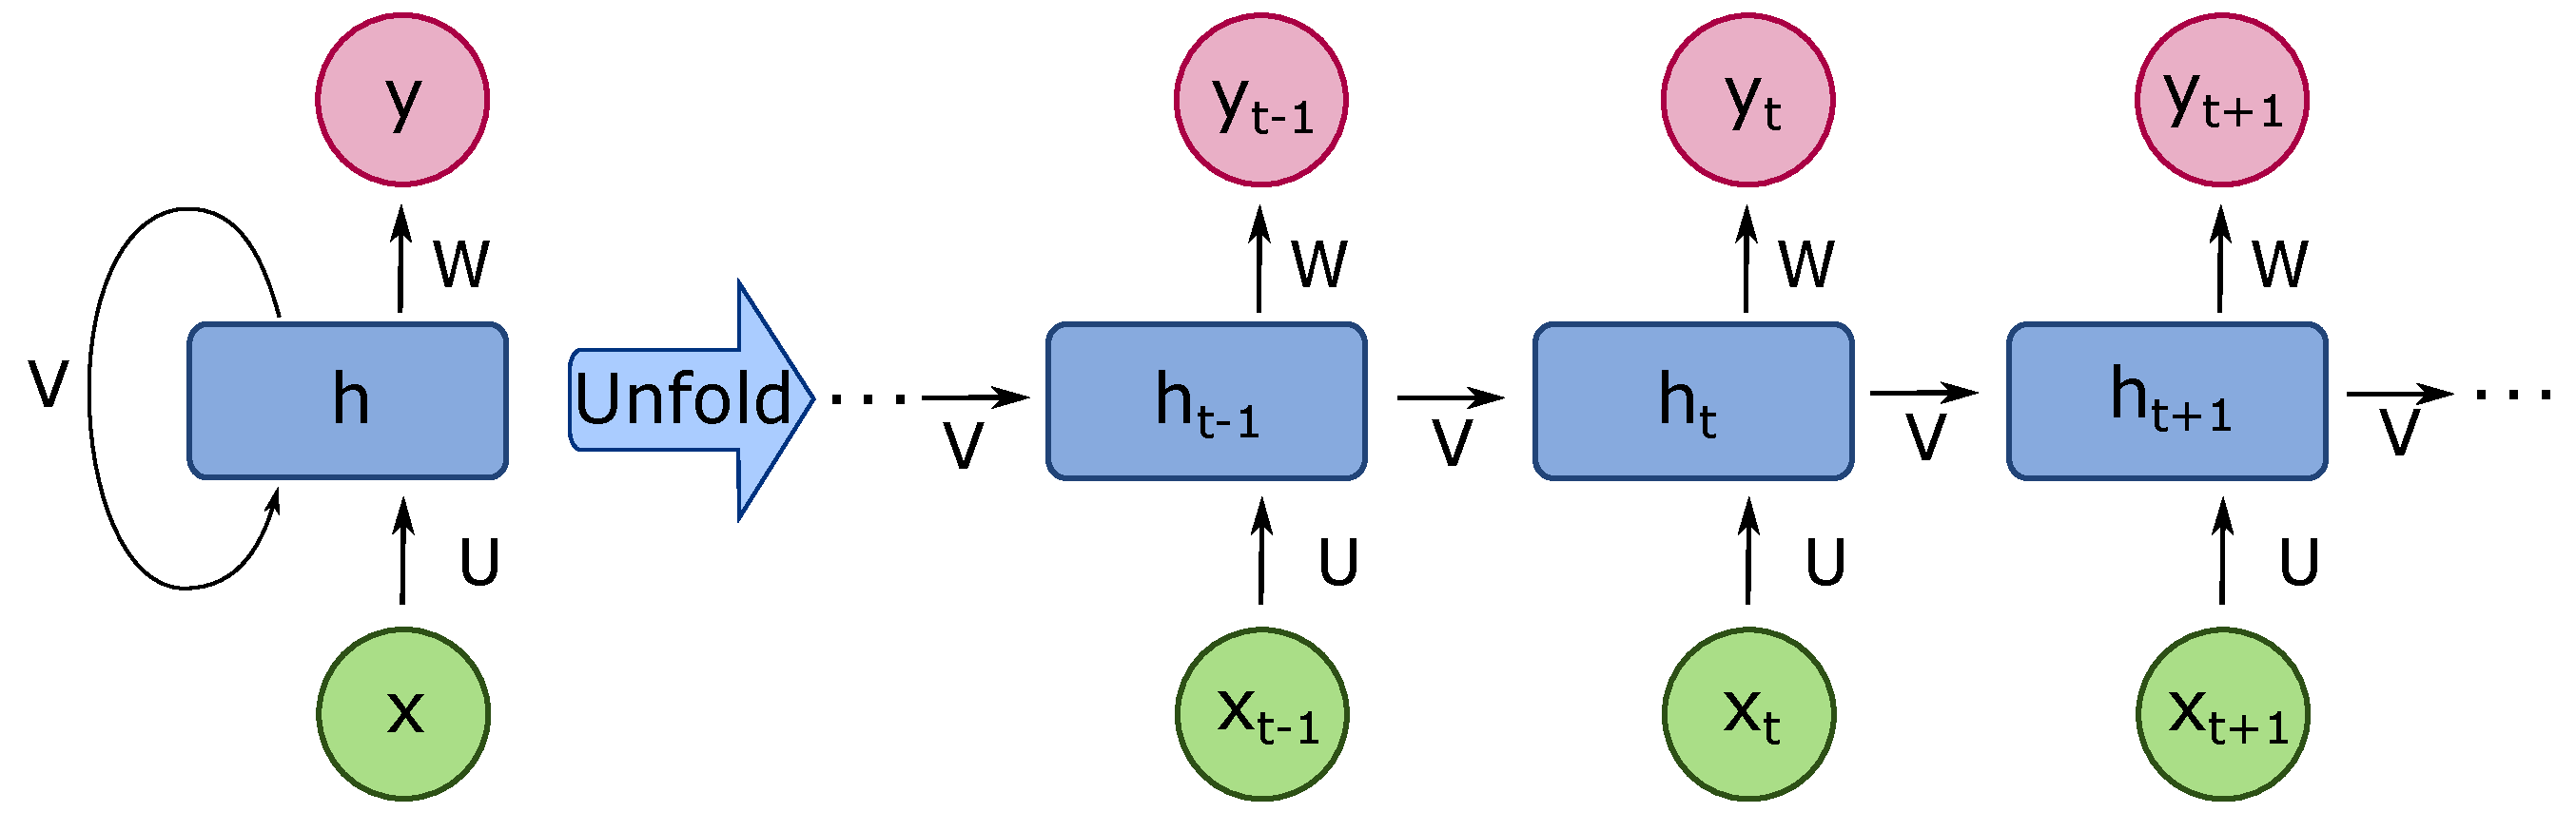
\includegraphics[width=.7\linewidth]{figures/3_theoretical_background/deep learning/rnn.pdf}
    \fignote{Adapted from \href{https://commons.wikimedia.org/wiki/File:Recurrent_neural_network_unfold.svg}{RNN - Wikimedia}}
    \label{fig:rnn}
\end{figure}

\subsubsection{Long Short-Term Memory (LSTM)}
\label{sec:lstm}

A \ac{LSTM} is an evolution of \ac{RNN} designed to mitigate vanishing gradients, allowing the model to capture long-term dependencies in sequential data \citep{graves2012long}. \acs{LSTM}s introduce a special cell structure (see Figure \ref{fig:lstm}) that includes input, forget, and output gates, allowing the model to control the flow of information and retain or discard information as needed.

\begin{figure}[ht!]
    \centering
    \caption{Diagarm of a Long Short-Term Memory model.}
    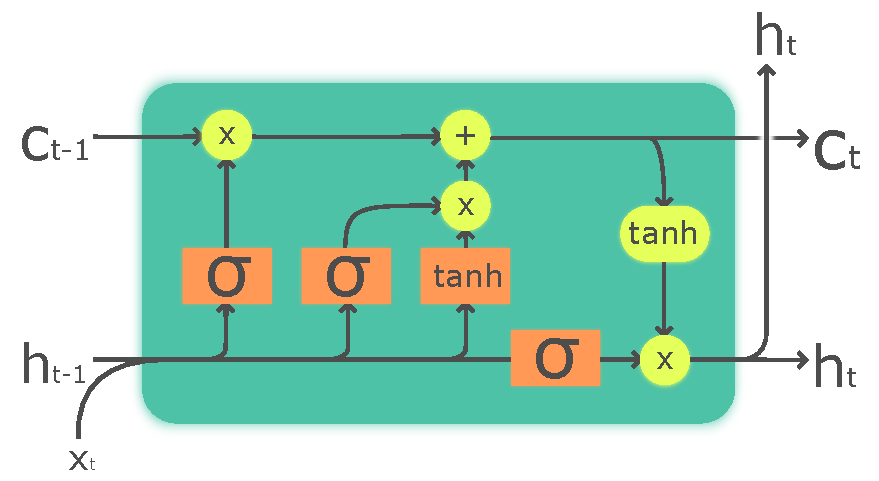
\includegraphics[width=.7\linewidth]{figures/3_theoretical_background/deep learning/lstm.pdf}
    \fignote{Adapted from \href{https://commons.wikimedia.org/wiki/File:The_LSTM_Cell.svg}{LSTM - Wikimedia}}
    \label{fig:lstm}
\end{figure}

The basis of the \ac{LSTM} is the cell state ($C_t$), a data line that runs through the entire chain and is protected by three gates that regulate what enters and what leaves. The Forget Gate ($\sigma$) decides, based on the current input ($x_t$) and the previous hidden state ($h_{t-1}$), which information from $C_{t-1}$ will be discarded or retained. Next, the Input Gate (composed of a Sigmoid $\sigma$ and a $\tanh$) determines which new data is important and adds it to the state cell. The new cell state ($C_t$) is then a combination of the old memory (filtered by the Forgetting Gate) and the new information (added by the Input Gate). Finally, the Output Gate ($\sigma$) decides which parts of $C_t$ (scaled by a tanh function) will be exposed as the hidden state ($h_t$) for the next time step, which is the actual output of the \ac{LSTM} unit to the subsequent layer and the next time step, completing the memory and prediction cycle.

A common variation of this architecture is the \acf{GRU}, which simplifies the LSTM by merging the forget and input gates into a single ``update gate'' and combining the cell state and hidden state \citep{cho2014learning}. This results in a more computationally efficient model with fewer parameters while maintaining similar performance in many tasks. Furthermore, the \acf{BiGRU} enhances this by processing the sequence in both forward and backward directions simultaneously \citep{schuster1997bidirectional}. This allows the model to capture context from both past and future states at any given time point, which is particularly useful for understanding the complete temporal evolution of a signal.

In \ac{RS}, \acs{LSTM}s and \acs{GRU}s have already been used for Crop Classification \citep{russwurm2023end} and Crop Yielding \citep{cheng2022wheat,jeong2022predicting}, due to the nature of time series in both applications. They are usually used pixel by pixel, i.e., each time series for each pixel is processed individually.

\subsubsection{Transformer}
\label{sec:transformer}

Transformer is a DL architecture originally developed for \acs{NLP}s tasks \citep{vaswani2017attention}, but which has been adapted for several other areas, including computer vision. This architecture has revolutionized the field of \ac{DL} due to its ability to capture long-range dependencies in sequential data, forming the basis for the construction of both commercial \acs{LLM}s such as ChatGPT \citep{openai2024gpt4technicalreport} and open source models such as Gemma \citep{gemmateam2025gemma3technicalreport}.

\begin{figure}[ht!]
    \centering
    \caption{Diagram of a Transformer model.}
    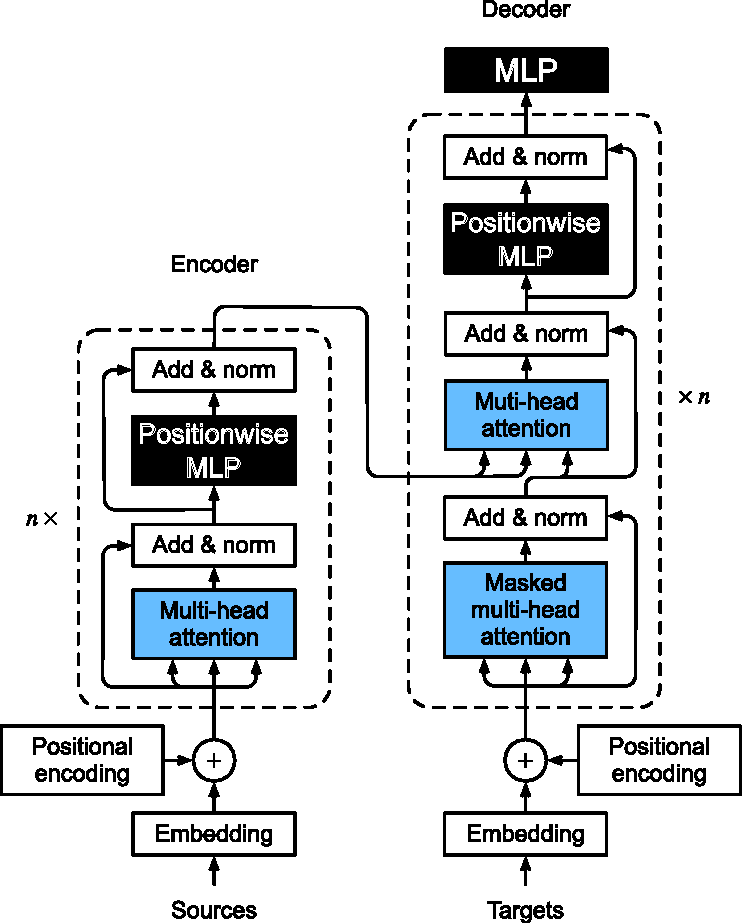
\includegraphics[width=0.7\linewidth]{figures/3_theoretical_background/deep learning/transformer.pdf}
    \fignote{Adapted from \href{https://pt.d2l.ai/chapter_attention-mechanisms/transformer.html/}{Dive into Deep Learning}}
    \label{fig:transformer}
\end{figure}

The model works by converting and processing data sequences through two interconnected structures, the Encoder (left) and the Decoder (right), which operate in $N$ repeated layers. The process begins by converting the inputs and targets into embeddings that are added (or concatenated, depending on the implementation) to a positional encoding to preserve the order of the elements. In the Encoder, Multi-head attention mechanisms simultaneously analyze the relationships between all parts of the input to create a rich representation of the context, which is refined by MLPs and normalizations for each point in the series. This contextualized representation is then sent to the Decoder, which combines the history of what has already been generated (using Masked multi-head attention to prevent access to future words) with the information coming from the Encoder, processing everything to generate the probability of the next output through a final \ac{CNN} (see graphically in Figure \ref{fig:transformer}).

Transformers were used in \ac{RS}, especially through some variations, such as the Vision Transformer (ViT) \citep{lin2023mmst} and the adapted \ac{BERT} \citep{shravan2024sits}, which will be explained later. In addition, the attention mechanism introduced by Transformers has been incorporated into several \ac{DL} architectures to improve the ability to capture spatial and temporal dependencies in \ac{RS} data.

\subsubsection{Vision Transformer (ViT)}

\Acf{ViT} is an adaptation of the Transformer architecture (see Setion \ref{sec:transformer}) for computer vision tasks such as image classification and semantic segmentation \citep{dosovitskiy2020image}. \ac{ViT} divides an image into small patches (e.g., $16\times16$ pixels), which are then flattened and transformed into embeddings, similar to words in \ac{NLP}. These embeddings are summed (or concatenated) with a positional encoding to preserve the spatial information of the patches before being fed into the Transformer model. The rest of the architecture follows the Transformer pattern, with Multi-head attention layers and \ac{MLP}s to process the embeddings of the patches and capture the relationships between them (see Figure \ref{fig:vit}), however, since the goal is not to generate a new image, the decoder is not used (which makes the architecture a subclass of Transformers called ``encoder-only'').


\begin{figure}[ht!]
    \centering
    \caption{Diagram of a Vision Transformer model.}
    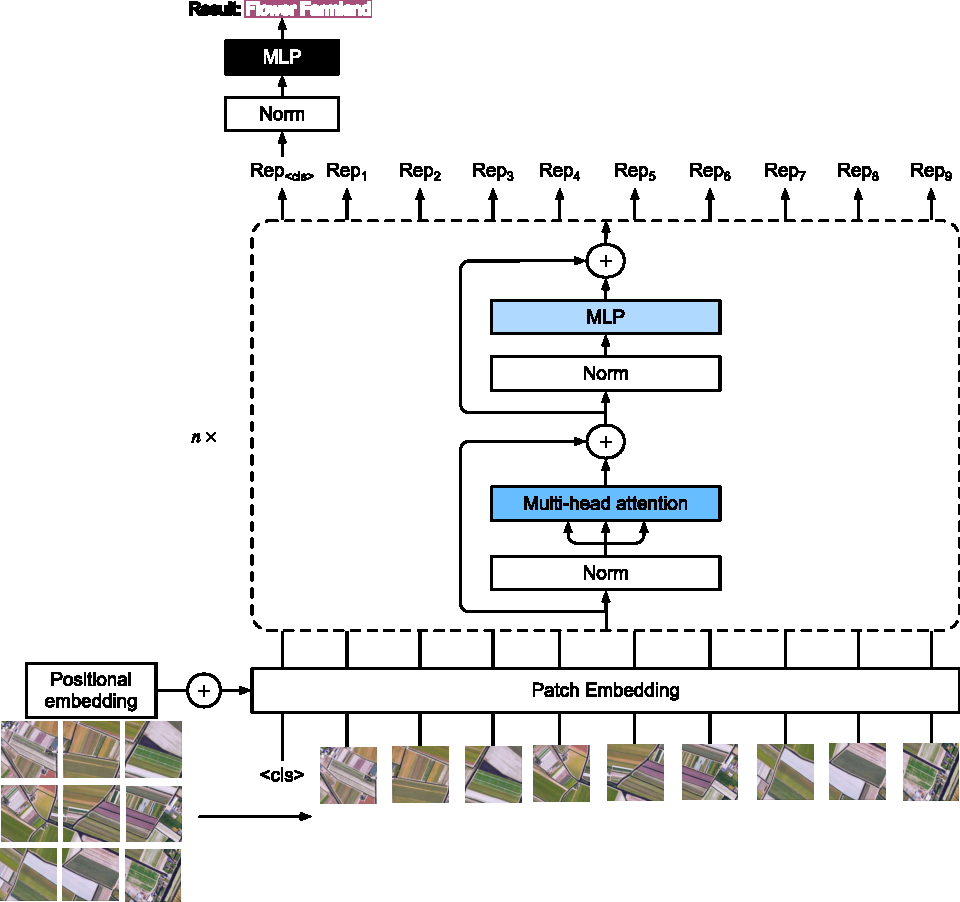
\includegraphics[width=0.7\linewidth]{figures/3_theoretical_background/deep learning/vit.pdf}
    \fignote{Adapted from \href{https://d2l.ai/chapter_attention-mechanisms-and-transformers/vision-transformer.html}{Dive into Deep Learning}}
    \label{fig:vit}
\end{figure}

Several variations of \ac{ViT} have been proposed, such as Swin Transformer, which introduces hierarchical attention mechanisms to improve the ability to capture features at different scales called Shifted windows, much like what \ac{CNN} do with their convolutional and pooling layers. The central idea is to subdivide the image several times, but each subdivision has its grid shifted relative to the previous one, allowing the model to capture both local and global features efficiently. A variation widely used in \ac{RS} is SwinNet, which combines the Swin Transformer as an encoder with an \ac{FCN}-based decoder (see Section \ref{sec:fcn}) to perform semantic segmentation.

\subsubsection{Bidirectional Encoder Representations from Transformers (BERT)}

\Acf{BERT} is a \ac{DL} model based on the Transformer architecture (see Section \ref{sec:transformer}) designed for NLP tasks \citep{devlin2019bert}. \ac{BERT} is trained using an unsupervised pre-training approach, where the model learns to predict masked words in a sentence (Masked Language Modeling) and to predict the next sentence in a pair of sentences (Next Sentence Prediction). It is known that predicting the next word is not necessary \citep{liu2019roberta}. This approach allows \ac{BERT} to capture the bidirectional context of words, considering both the context to the left and right of a word in a sentence. Subsequently, the model can be fine-tuned for a specific task, such as grammatical classification using less labeled data (see Figure \ref{fig:bert}). Note that details about \ac{SSL} pre-training, which is the case with BERT, will be better addressed in Section \ref{sec:ssl_contextualization} (the BERT pre-training, which is a Masked Modeling pre-training, it is discussed in details in Section \ref{sec:ssl_mim}).

\begin{figure}[ht!]
    \centering
    \caption{Diagram of a Bidirectional Encoder Representations from Transformers model.}
    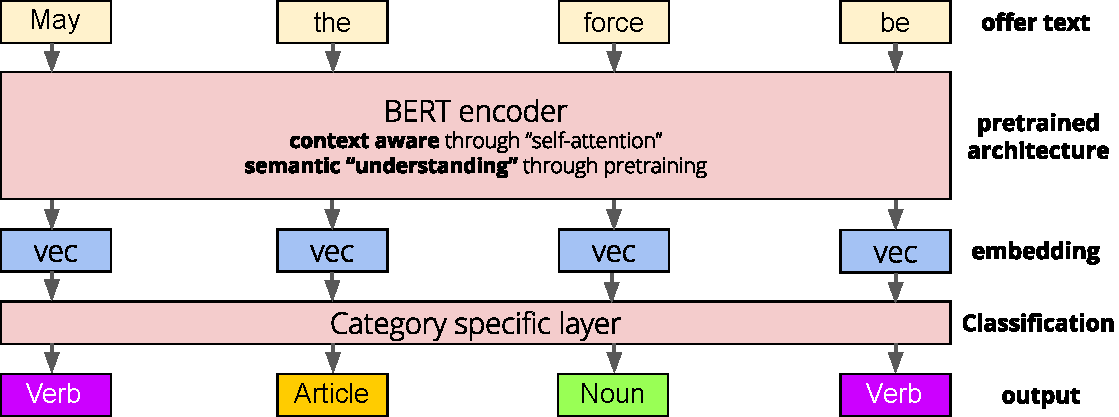
\includegraphics[width=.85\linewidth]{figures/3_theoretical_background/deep learning/bert.pdf}
    \fignote{Adapted from \href{https://dida.do/projects/numeric-attribute-extraction-from-product-descriptions}{Dida.do}}
    \label{fig:bert}
\end{figure}

Although \ac{BERT} was designed to handle \ac{NLP} data, its basic idea of Bidirectional Encoder has been adapted for other purposes such as DNA analysis \citep{zhou2025dnabert}, protein analysis \citep{brandes2022proteinbert}, and item recommendation \cite{sun2019bert4rec}. In Remote Sensing, variations of \ac{BERT} have been adapted to process \ac{SITS}, using spectral bands linearly projected directly into the \ac{BERT} Encoder.

\subsubsection{Mamba and the post-Transformer question}

Although Transformers (see Section \ref{sec:transformer}) have established the state of the art in several tasks, their architecture presents a fundamental limitation: the computational and memory complexity of the self-attention mechanism scales quadratically ($O(L^2)$) with respect to the sequence length $L$. There are even ethical discussions about the environmental impacts caused by LLMs, which almost entirely use Transformers. Which model performs as well as a Transformer but is linear ($(O(L))$) or linear-logarithmic ($(O(L\times \log L))$) is perhaps the major current question in the field of Machine Learning, with the other major question being whether such a model can even exist.

One attempt to address this is through state-space models (SSMs), with the Mamba model as its main representative. Mamba introduces a selection mechanism that allows the model to filter out irrelevant information and focus on specific contextual data, operating with linear complexity ($O(L)$).

\begin{figure}[ht!]
    \centering
    \caption{Diagram of a Mamba model.}
    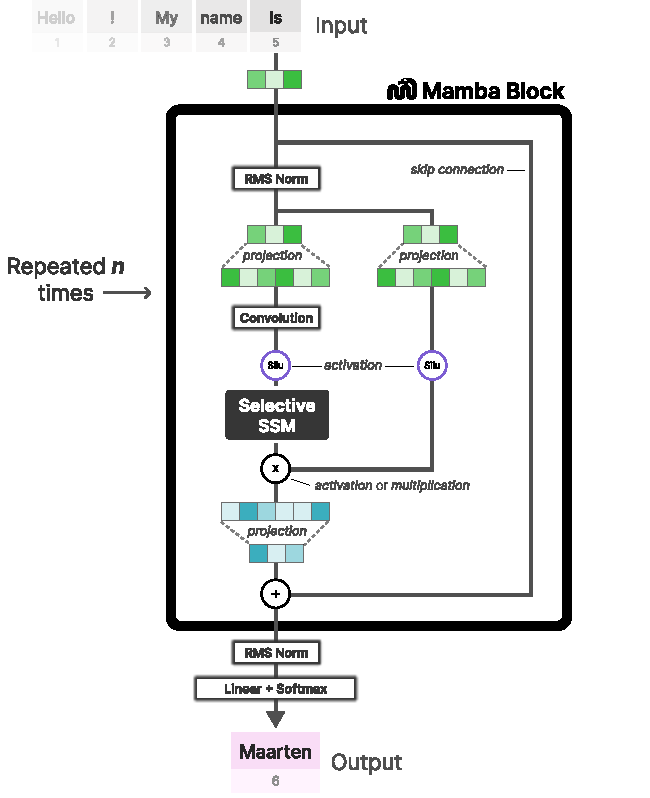
\includegraphics[width=0.75\linewidth]{figures/3_theoretical_background/deep learning/mamba.pdf}
    \fignote{Adapted from \href{https://www.maartengrootendorst.com/blog/mamba/}{
Maarten Grootendorst Blog}}
    \label{fig:mamba}
\end{figure}

The Mamba architecture is based on Selective State Space Models (S6), which allow model parameters to be functions of the input, giving it a contextual reasoning capability comparable to that of Transformers. In the field of computer vision, this approach gave rise to Vision Mamba (Vim) \citep{zhu2024vision} and VMamba \citep{liu2024vmamba}, which adapt linear scanning to two-dimensional data through the Cross-Scan Module, allowing the model to capture spatial dependencies in images without the high cost of global attention.
\section{Self-Supervised Representation Learning}
\label{sec:ssl_contextualization}

% \fromsurvey{In a scenario where the efficacy of transfer learning via fine-tuning from pretrained supervised networks is limited due to geographical domain shift \citep{nyborg2022timematch}, more robust strategies are required, such as knowledge distillation \citep{bazzi2020distilling}, domain adaptation \citep{wang2021phenology} or self-supervised learning \citep{yuan2020self,yuan2022sits,xu2024self}. This is aggravated by the lack of vast labeled datasets (see Table \ref{tab:context_labeled_datasets}), which prompted research in the field of Deep Learning for \ac{RS} seems to move towards unsupervised representation learning. In this sense, Foundational Models (FMs) are one of the most prominent family of representational methods, capable of learning richer representations from multi-modal data, enabling zero-shot predictions on a variety of tasks. FMs seem better suited for remote sensing tasks due to the lack of labeled data \citep{huo2025remote}, but there are many challenges, including data acquisition, training efficiency, data shift, and practical application challenges to use FMs in real-world scenarios \citep{yin2025fms}.}

%\fromsurvey{As described by \citep{liu2021self}, the two most common ways of computing such representations directly from unlabeled data are: (i) generative modeling; and (ii) self-supervision. In the remaining sections of this manuscript, we focus on the latter approach and its application to agricultural tasks.}


\Acf{SSL} \fromsurvey{consists of extracting supervision signals from unlabeled data, usually widely available in \ac{RS}. These procedurally computed labels are then used for pretraining learning models, which can be fine-tuned for downstream tasks using smaller amounts of labeled data \citep{balestriero2023cookbookselfsupervisedlearning}. Several visual \ac{SSL} methods \citep{he2021maskedautoencodersscalablevision} are inspired by techniques used in the pretraining phases of \acs{LLM}s such as \ac{BERT} \citep{devlin2019bert}, wherein the model is trained to recover masked words from the context of neighboring words.}

It is well known in the literature that Transfer Learning between supervised trainings does not work very well for \ac{RS}, given that the models do not generalize well between different regions, especially in agriculture, since there are climatological, soil, and even subspecies differences, where the same crop class has different subspecies for each region. Furthermore, supervised datasets are scarce (as demonstrated in \autoref{tab:context_labeled_datasets}). Therefore, \ac{SSL} proves to be a particularly useful tool for agricultural \ac{RS}, considering all these problems described, in addition to the abundance of unlabeled data, since satellites are constantly acquiring data, and there are several publicly available missions (as demonstrated in \autoref{tab:context-satellites}), plus the main characteristic of \ac{SSL} of learning intrinsic features of the target data.

\newcommand{\figscale}{0.5}

\begin{figure}[ht!]
    \centering
    \caption{Overview of the self-supervised pretraining and finetuning process.}
    \begin{subfigure}[c]{0.975\columnwidth}
        \centering
        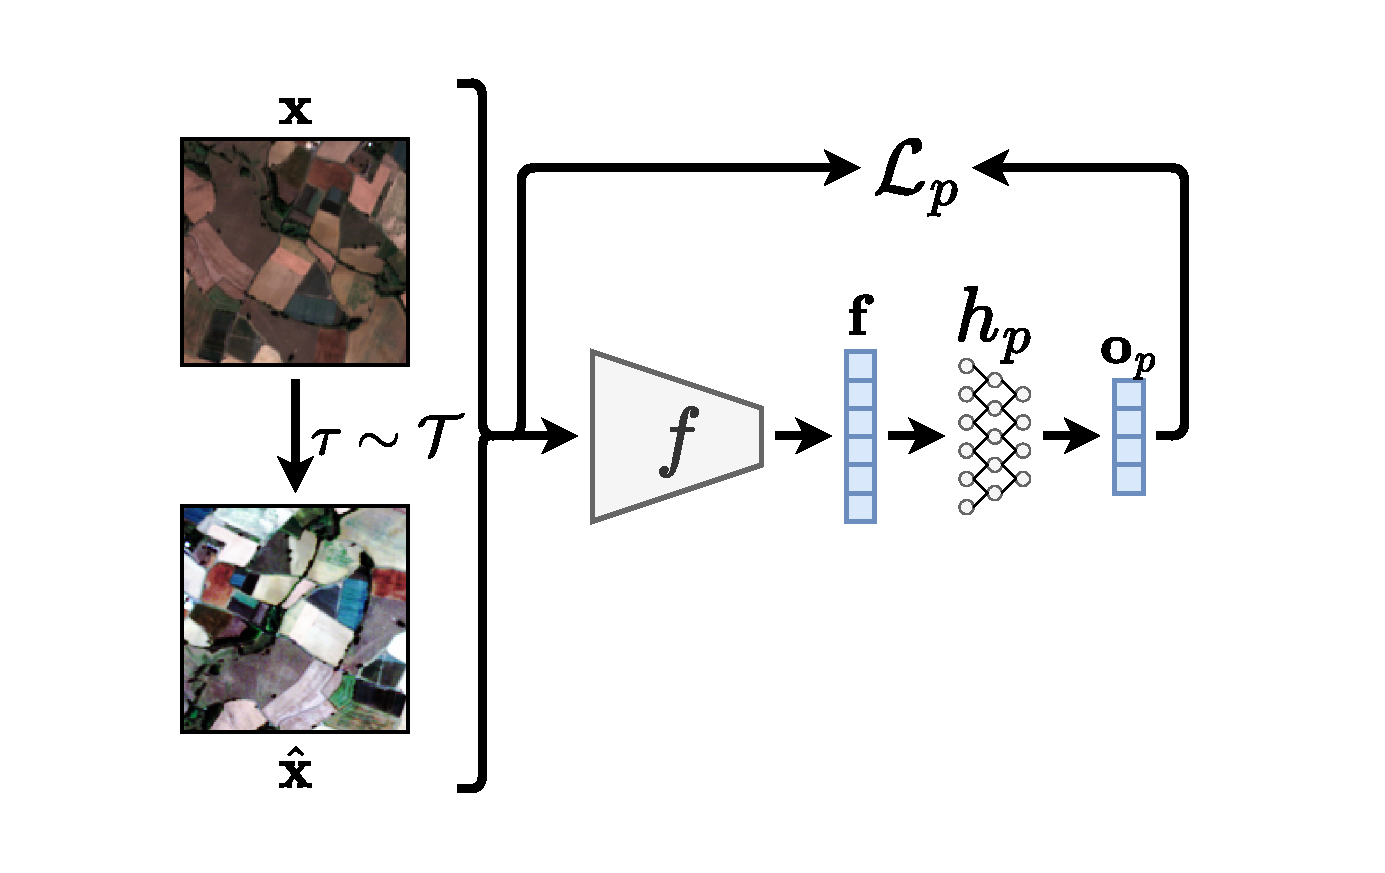
\includegraphics[clip,trim=1.15in 0.45in 0.45in 0.45in,scale=\figscale]{figures/3_theoretical_background/ssl/representation_learning_pre-training.pdf}
        \caption{\fromsurvey{}}
        \label{fig:ssl_overview_pre-training}
    \end{subfigure}
    \\
    \begin{subfigure}[c]{0.975\columnwidth}
        \centering
        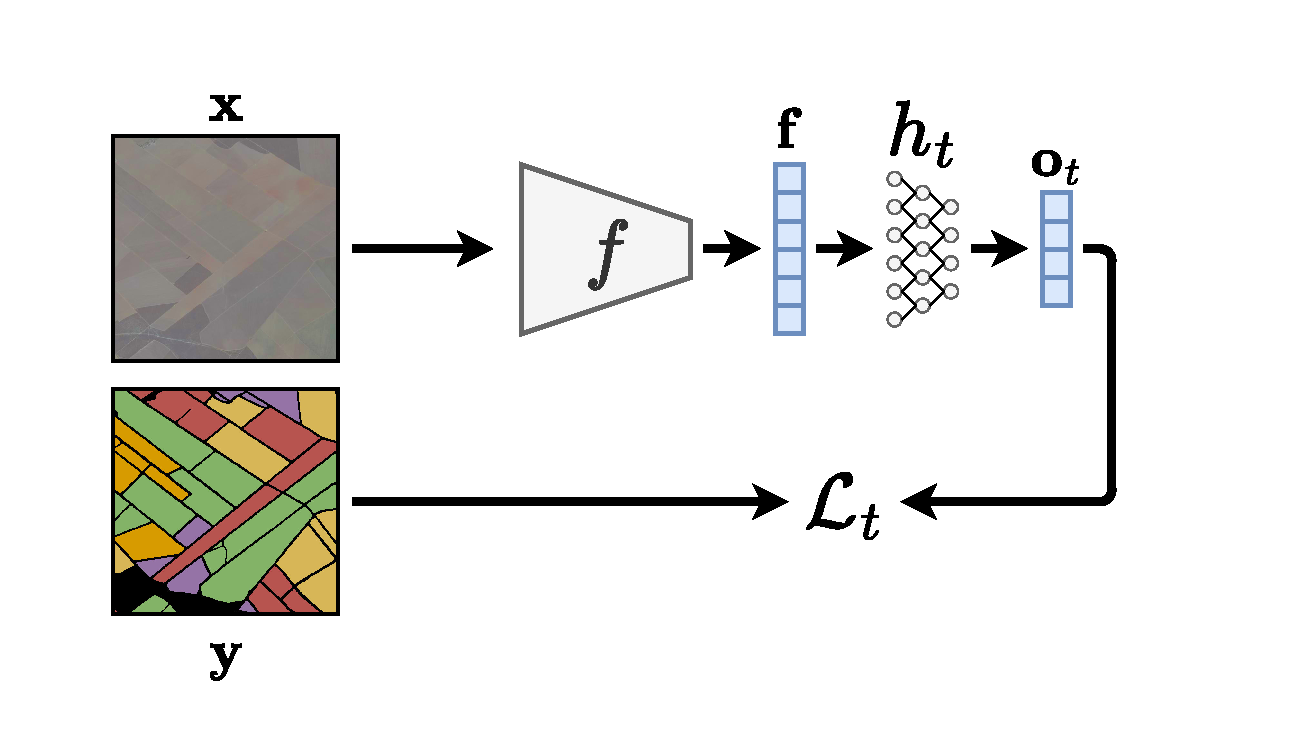
\includegraphics[clip,trim=0.75in 0.45in 0.45in 0.45in,scale=\figscale]{figures/3_theoretical_background/ssl/representation_learning_finetuning.pdf}
        \caption{\fromsurvey{}}
        \label{fig:ssl_overview_finetuning}
    \end{subfigure}
    \fignote{Overview of the self-supervised pretraining process (a) of a model $f$ using a loss $\mathcal{L}_p$ (a), followed by a fine-tuning step (b) to a target labeled task via a loss $\mathcal{L}_t$ (b). One should notice that only the backbone $f$ is maintained, while the pretraining head $h_p$ is swapped for a novel, randomly initialized target task head $h_t$.}
    \label{fig:ssl_overview}
\end{figure}

\fromsurvey{Visual \ac{SSL} began with transform prediction, i.e., procedurally augment an image using geometric, color, or masking transforms and train a model to predict which transform parameter was applied to that image. More formally, given an image $\mathbf{x}$, one can apply a randomly sampled transform $\tau \sim \mathcal{T}$ to generate the transformed version $\hat{\mathbf{x}}$. $\hat{\mathbf{x}}$ can then be passed forwarded through a backbone model $f$, yielding feature vector $\mathbf{f}$. The backbone $f$ and head $h$ are, therefore, trained to predict which randomly sampled transformation $\tau$ was applied to $\mathbf{x}$. For instance, classifying which rotation \citep{gidaris2018unsupervised} or affine transform \citep{kanazawa2016warpnet} a given image underwent. Some tasks not commonly used as data augmentations were also used, like jigsaws on the image, and the pretext task was to classify the correct order for the reconstruction of the original image \citep{kanazawa2016warpnet}. A prototypical transform prediction \ac{SSL} approach can be seen in Figure \ref{fig:ssl_transform}.}

\begin{figure}[ht!]
    \centering
    \caption{Overview of transform prediction self-supervised learning}
    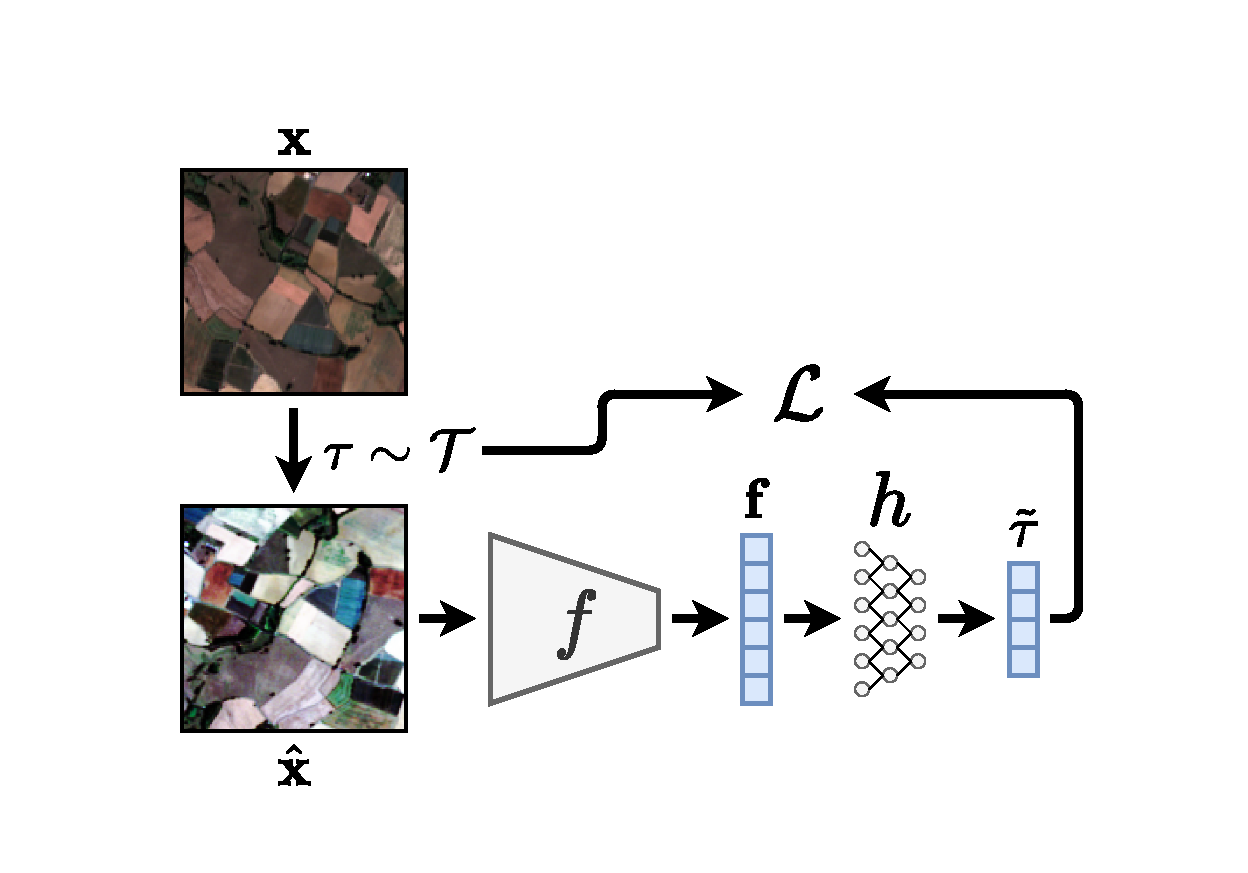
\includegraphics[clip,trim=0.75in 0.45in 0.45in 0.45in,scale=\figscale]{figures/3_theoretical_background/ssl/transform_prediction.pdf}
    \fignote{The original image $\mathbf{x}$ is transformed using $\tau \sim \mathcal{T}$ into $\hat{\mathbf{x}}$, which is fed through the networks $f$ and $h$ to predict $\tilde{\tau}$. A classification or regression loss $\mathcal{L}$ is then used to enforce that $\tilde{\tau} \approx \tau$.}
    \label{fig:ssl_transform}
\end{figure}

\fromsurvey{Little work has been done on transform prediction for \ac{RS}. \cite{wen2021rotation} used rotation prediction for object recognition using \ac{SAR} data, improving few-shot recognition performance. Again, \cite{xu2021self} employed the same methodology for object recognition for optical data. The latter also notes that doing this during semi-supervised hybrid training (see more in Section \ref{sec:ssl_semi}) presents slightly better results.}

\subsection{Similarity-based Self-Supervision}
\label{sec:ssl_similarity}

\fromsurvey{However, transform prediction \ac{SSL} has severe limitations, such as generating covariant embeddings with respect to the transformations applied to the input, as well as unrepresentative representations caused by the backbone learning to identify shortcuts instead of relevant features \citep{minderer2020automatic}. 
In order to extract more representative representations, \ac{SSL} has migrated to similarity-based techniques. Such methods approximate embeddings for multiple views of a single image, rendering the backbones invariant to these data augmentations instead of covariant to them. By doing this, the pretraining procedure encourages the representation to discriminate across instances, generating more sparse embeddings.}


\fromsurvey{Figure \ref{fig:ssl_sim} depicts a similarity-based \ac{SSL} strategy. From a single image $\mathbf{x}$, two views $\mathbf{x}_1 = \tau_1(\mathbf{x})$ and $\mathbf{x}_2 = \tau_2(\mathbf{x})$ are generated by applying two randomly sampled transformations $\tau_1, \tau_2 \sim \mathcal{T}$. $\mathbf{x}_1$ and $\mathbf{x}_2$ are then passed through a backbone $f$, yielding the feature representations $\mathbf{f}_1$ and $\mathbf{f}_2$, which are then passed through a projection head $h$, resulting in the projected vectors $\mathbf{p}_1$ and $\mathbf{p}_2$. The whole ensemble is then trained by encouraging similarity between $\mathbf{p}_1$ and $\mathbf{p}_2$ via a similarity loss $\mathcal{L}_{sim}$.}


\begin{figure}[ht!]
    \centering
    \caption{Overview of similarity self-supervised pretraining.}
    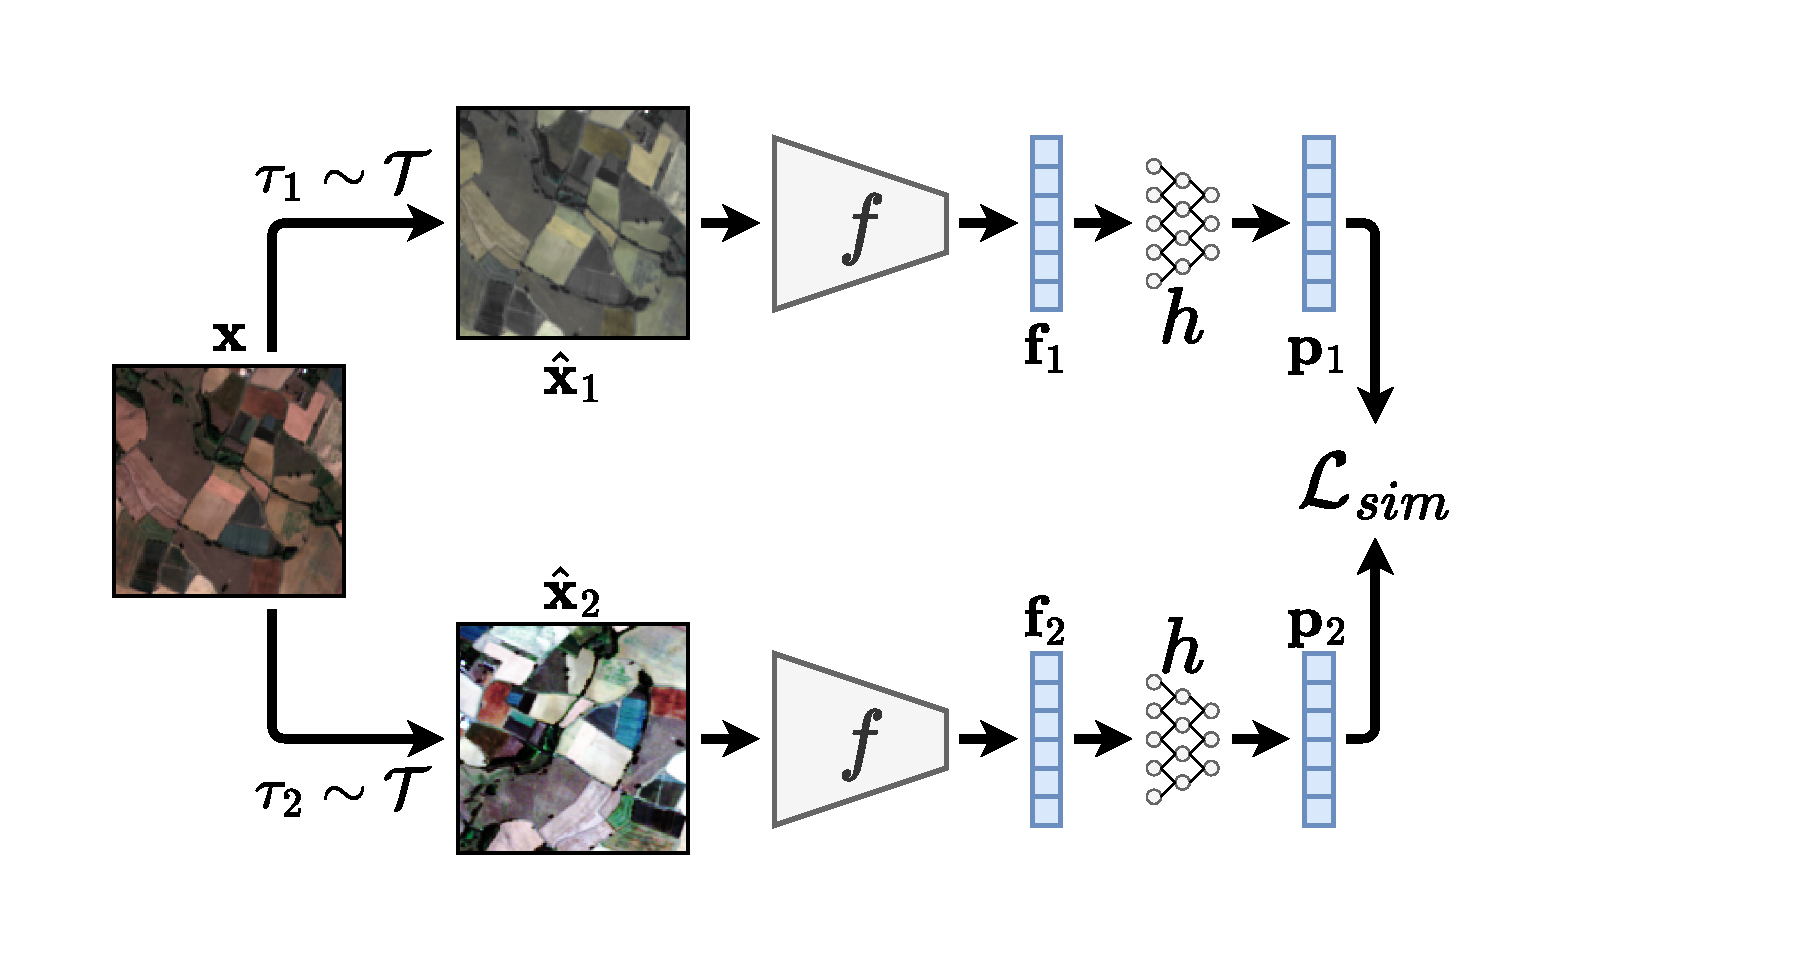
\includegraphics[clip,trim=0.75in 0.45in 2.4in 0.45in,scale=\figscale]{figures/3_theoretical_background/ssl/similarity.pdf}
    \fignote{ Two views $\mathbf{x}_1$ and $\mathbf{x}_2$ from a sample $\mathbf{x}$ computed using the transformations $\tau_1$ and $\tau_2$ are passed through a backbone $f$ and a projection head $h$, yielding projections $\mathbf{f}_1$ and $\mathbf{f}_2$, which are then encouraged to be similar via a similarity loss $\mathcal{L}_{sim}$.}
    \label{fig:ssl_sim}
\end{figure}

\subsubsection{Contrastive Self-Supervised Learning}
\label{sec:ssl_contrastive}

\fromsurvey{In order to avoid the mode collapse problem caused by enforcing similarity between different views of the same image (positive pairs), contrastive \ac{SSL} methods employ very large batch sizes to hold several negative pairs in each learning iteration. Thus, pretraining such contrastive methods may require several \acs{GPU}s with large \ac{VRAM} capacity. \ac{SimCLR} \citep{chen2020simple}, for instance, is a highly influential contrastive \ac{SSL} strategy that requires very large batch sizes. In this approach, the normalized temperature-scaled cross-entropy loss (NT-Xent) is used, leveraging negative pairs from other samples in the batch and achieving a top-1 \ac{OA} of 79.8\% in ImageNet.}

\fromsurvey{Multiple strategies employ smarter ways to leverage negative pairs to avoid the need for large batch sizes. \Acf{MoCo} \citep{he2020momentum, chen2020improved, chen2021empirical} uses a dictionary implemented with a Round Robin queue that stores previously batched negative samples. This makes it possible to decouple the problem of the number of negative pairs from the batch size. In \ac{MoCo}, the key encoder is updated smoothly using a moving average of the query encoder (momentum). This approach leverages the InfoNCE loss to minimize the distance between a query and its positive key and maximize the distance to negative keys, resulting in 81\% in ImageNet in its more recent version.}

\fromsurvey{Another approach to addressing large batch sizes was taken by \cite{caron2020unsupervised} propose \Acf{SwAV} as a pretraining \ac{SSL} strategy. \ac{SwAV} works by predicting online clusters for each augmented multiresolution view of the images via the Sinkhorn-Knopp algorithm. The method does not use direct comparisons between embeddings generated by the augmentations, which eliminates the need for large batch sizes. Instead of traditional instance-wise contrastive learning, \ac{SwAV} is understood as a contrastive clustering approach. As a result, \ac{SwAV} achieved 75.3\% in the same test procedure as \ac{SimCLR} and \ac{MoCo}. \ac{SwAV} was the first \ac{SSL} method to overcome supervised pretraining in ImageNet in transfer learning tasks to other downstream RGB datasets.}

\fromsurvey{Barlow Twins \citep{zbontar2021barlow} use negative samples from the batch itself without the need for a large batch size. This is achieved via a more thorough grid search on the optimizer's hyperparameters. Using a Siamese network that processes two augmented views of the data, Barlow Twins generates a cross-correlation matrix of the augmented embeddings -- twins -- of the batch and trains the network to approximate the identity matrix. By approximating the values of the main diagonal to 1, it forces the invariance of the augmentations. By approximating the other values of the matrix to 0, it avoids collapse. The method has performance comparable to previous methods, including some non-contrastive methods (see Section \ref{sec:ssl_non_contrastive}).}

\fromsurvey{\Acf{SeCo} \citep{yao2021seco} specifically addresses video tasks such as action recognition, untrimmed activity recognition, and object tracking. For this, the models are pretrained on videos, and three pretrained tasks were designed for this: intra-frame discrimination, which determines whether two image patches belong to the same video frame, inter-frame discrimination, which determines whether two image patches belong to the same video, and temporal order validation, which checks whether a sequence of patches is in the correct temporal order. This leads to an improvement in action recognition \ac{OA} of 2.96\% and 6.47\% on UCF101 and HMDB51 against supervised ImageNet pretraining.}

\fromsurvey{Traditional contrastive \ac{SSL} has been employed in RS tasks. \cite{ayush2021geography} adapted \ac{MoCo} by adjusting its augmentations that originally were designed for natural images. For this, temporal views of the same image are used as positive pairs, while images from different positions are used as negative samples. In addition, the prediction of the geolocation of the region of interest is incorporated into the pretext task. For this, the coordinates of the images are previously clustered using K-Means, and the prediction of which cluster each image belongs to is added to the loss. Results indicate that the method outperforms \ac{MoCo} in \ac{RS} tasks. \Acf{DeCUR} \citep{wang2024decoupling} follows the Barlow Twins paradigm, separating inter-modal representations (shared across data modalities) and intra-modal representations (unique within each data modality), enabling the model to learn both shared characteristics and modality-specific features. \ac{DeCUR} outperforms multiple \ac{SSL} methods designed for natural images in both classification and semantic segmentation of images. \ac{SeCo} \citep{yao2021seco} was also used in \ac{RS} \citep{Manas_2021_ICCV} settings, in this case with very few modifications. The results obtained were better in several downstream tasks compared to \ac{MoCo}. These results reinforce the need for domain-specific augmentations in visual \ac{SSL}.}

\subsubsection{Non-Contrastive Self-Supervised Learning}
\label{sec:ssl_non_contrastive}

\fromsurvey{More recently, techniques that do not depend on negative samples have emerged, which completely get rid of the need for memory to store them, either in large batches or in other structures. \Acf{BYOL} \citep{grill2020bootstrap} showed that negative pairs are not needed for avoiding mode collapse. \ac{BYOL} employs two networks: \textit{online} and \textit{target}; wherein the \textit{online} network is trained in a traditional fashion and the \textit{target} is updated with an exponential moving average. The \textit{target} network incorporates a prediction head that projects the embeddings to avoid the collapse of the representations, getting 79.6\% on the same test of \ac{SimCLR}, but using a ResNet with 200 layers. \Acf{DINO} \citep{caron2021emerging} was heavily inspired by \ac{BYOL}, transforming it into a complete knowledge distillation architecture. \ac{BYOL} is heavily focused on optimizing convolutional networks such as ResNet, while \ac{DINO} shows that \acs{ViT}s, show interesting emergent properties of their pretraining. \acs{ViT}s pretrained with \ac{DINO} have internal activations more present in the most informative pixels in the images representing the classes, even with pretraining without labels, achieving 77\% in ImageNet with \acs{ViT}-B/8.}

\fromsurvey{\Acf{SimSiam} \citep{chen2021exploring} considerably simplified non-contrastive \ac{SSL} by approximating embeddings through a Siamese architecture, with one of the branches having an \ac{MLP} as a predictor, and the other applying a stop-gradient operation. The authors describe the method in several ways, including a \ac{SwAV} without online clustering and a \ac{BYOL} without an exponential moving average of the weights, achieving performance very close to contrastive methods. Compared to other non-contrastive methods, \ac{SimSiam} is minimalist, only including what really makes similarity-based \ac{SSL} work without negative pairs. \cite{pototzky2022fastsiam} further improved \ac{SimSiam} into \ac{FastSiam} by regularizing the pretraining by using multiple views instead of only two, achieving similar results, but with only a single \ac{GPU} used during training and a very small batch size.}

\fromsurvey{\cite{bardes2021vicreg} addressed mode collapse in another way, using two forms of regularization in the embeddings: a term that maintains the variance of each embedding dimension above a threshold and a term that decorrelates each pair of variables, creating the \Acf{VICReg} method. \ac{VICReg} does not use negative pairs, while also not using stop-gradient operations, achieving performances comparable to contrastive methods. \Acf{VICRegL} \citep{bardes2022vicregl} builds upon VICReg by adding a new branch to the network responsible for processing local visual information. Even though \ac{VICRegL} results in a 1.1\% drop in classification \ac{OA} in ImageNet, this strategy is shown to be more suited to semantic segmentation and detection tasks. VICRegL yields an 8.1\% mIoU improvement in Pascal VOC, showing that targeted \ac{SSL} pretraining can be better suited to downstream tasks other than image classification.}

\subsection{Masked Modeling}
\label{sec:ssl_mim}

\fromsurvey{Another group of widely used methodologies that draws inspiration directly from \ac{NLP} is \Acf{MM}, in which a portion of the input data for each sample is masked and the pretext task becomes reconstructing the original input data. A typical \ac{MM} approach can be seen in Figure \ref{fig:ssl_mim}. The original image $\mathbf{x}$ is initially sliced into patches, forming the patched image $\mathbf{w}$. A percentage of the patches is masked (hidden), forming $\hat{\mathbf{w}}$, while the masked pixels form the image comprising the invalid pixels $\mathbf{w}_i$. The valid patches are linearized, forming $\hat{\mathbf{w}}_v$ which is passed through the ViT backbone $f$ that serves as an encoder, resulting in the encoded representations $\mathbf{e}_v$. The masked patches are appended to $\mathbf{e}_v$, resulting in $\mathbf{e}_w$, which is passed through the decoder $g$. The output of the ensemble of networks is $\mathbf{d}_w$ representing an embedding with information about the reconstruction of the valid and invalid patches. From $\mathbf{d}_w$, only the originally masked patches are reconstructed in image $\tilde{\mathbf{w}}_i$, which is compared to $\mathbf{w}_i$ via a reconstruction loss $\mathcal{L}_{rec}$.}

\begin{figure}[ht!]
    \centering
    \caption{Overview of masked image self-supervised pretraining.}
    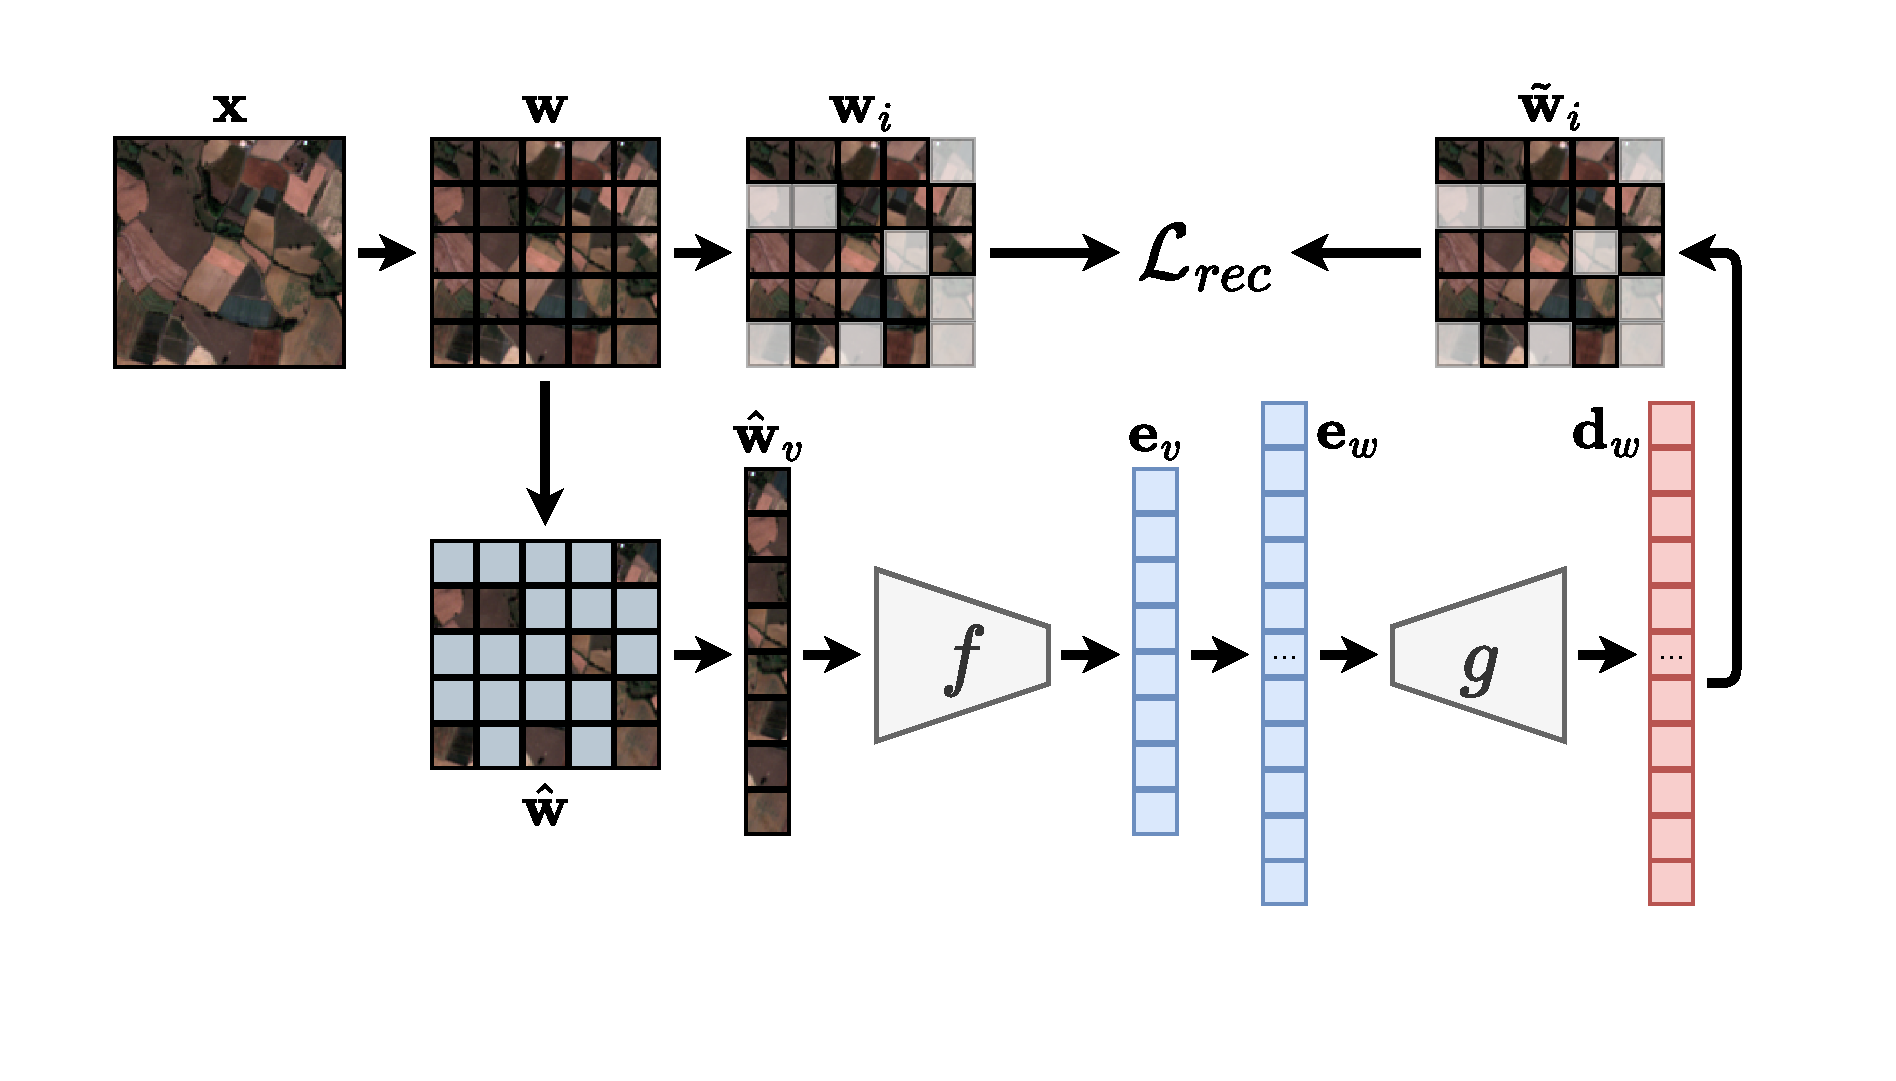
\includegraphics[clip,trim=0.55in 0.4in 0.95in 0.45in,scale=\figscale]{figures/3_theoretical_background/ssl/masked_image_modeling.pdf}
    \fignote{Initially, image $\mathbf{x}$ is windowed, forming $\mathbf{w}$, which yields the valid patch list $\hat{\mathbf{w}}_v$. The patches in $\hat{\mathbf{w}}_v$ are then passed through encoder $f$, resulting in the encoded vector $\mathbf{e}_v$, appended to reinsert the representations of the invalid (masked) patches, resulting in $\mathbf{e}_w$. $\mathbf{e}_w$ is then passed through the decoder $g$, resulting in the reconstruction embedding $\mathbf{d}_w$. From $\mathbf{d}_w$, the reconstruction of the masked patches $\tilde{\mathbf{w}}_i$ is compared to $\mathbf{w}_i$ via a loss $\mathcal{L}_{rec}$. Afterwards, $f$ is repurposed for fine-tuning to a downstream task.}
    \label{fig:ssl_mim}
\end{figure}

\fromsurvey{Following the \ac{MM} paradigm, \Acf{MAE} \citep{he2021maskedautoencodersscalablevision} masks patches from a ViT. The authors showed that the best strategy is to pretrain with 75\% of the patches randomly masked, achieving 76.6\% in ImageNet with a ViT-H/14. Furthermore, it was shown that reconstructing an image without masking patches results in ineffective pretraining, since it is not a complex enough task to force the networks to learn representative features. \Acf{SimMIM} \citep{xie2022simmim} is an approach that works as an advancement and simplification of \ac{MAE}, using direct regression of the RGB values of masked pixels and a lightweight linear decoder head, rendering it a highly efficient pretraining strategy.}

\fromsurvey{Generalist approaches for RS using the idea of data masking have also been developed. \cite{reed2023scale} adapted \ac{MAE} for this domain, introducing a positional encoding based on the spatial resolution of the images. In addition, their Scale-\ac{MAE} separately reconstructs low and high-frequency components using a Laplacian decoder, allowing multiscale learning, while the classic \ac{MAE} reconstructs only the original image. This makes Scale-\ac{MAE} more robust for remote sensing by dealing with multiple scales. The authors demonstrate the improvement in several downstream tasks, including also demonstrating embedding improvement via K-Nearest Neighbors analysis. \cite{xiong2024neural} extended the method based on the idea of neuroplasticity, being able to deal with any number of spectral bands and sensor modalities. Their approach uses a hyper-network-based dynamic weight generator that adjusts its architecture for new sensors, having as input the central reflectance value of each of the bands in addition to the images.}

\fromsurvey{More recent work uses a method that combines MIM with Similarity-based \ac{SSL}, in which views are approximated, but with some having patches of their data masked. Masked Siamese Network (MSN) \citep{assran2022masked} approximates two views of the same image through Negative Cosine Similarity. In the anchor view, some data is masked, while the target view undergoes more aggressive color and geometric augmentations, aiming to render the model invariant to them. Prior Matching for Siamese Networks (PMSN) \citep{assran2022hidden} demonstrated that, although the previous methods do not require pretraining labels, it is still assumed that the classes that exist in the datasets are approximately balanced. To address this, the authors modified the loss function to include a power-law in order to force a balancing of classes per batch, improving the performance on imbalanced data, but degrading the performance on balanced datasets.}

\begin{figure}[ht!]
    \centering
    \caption{\fromsurvey{Overview of masked image similarity self-supervised pretraining.}}
    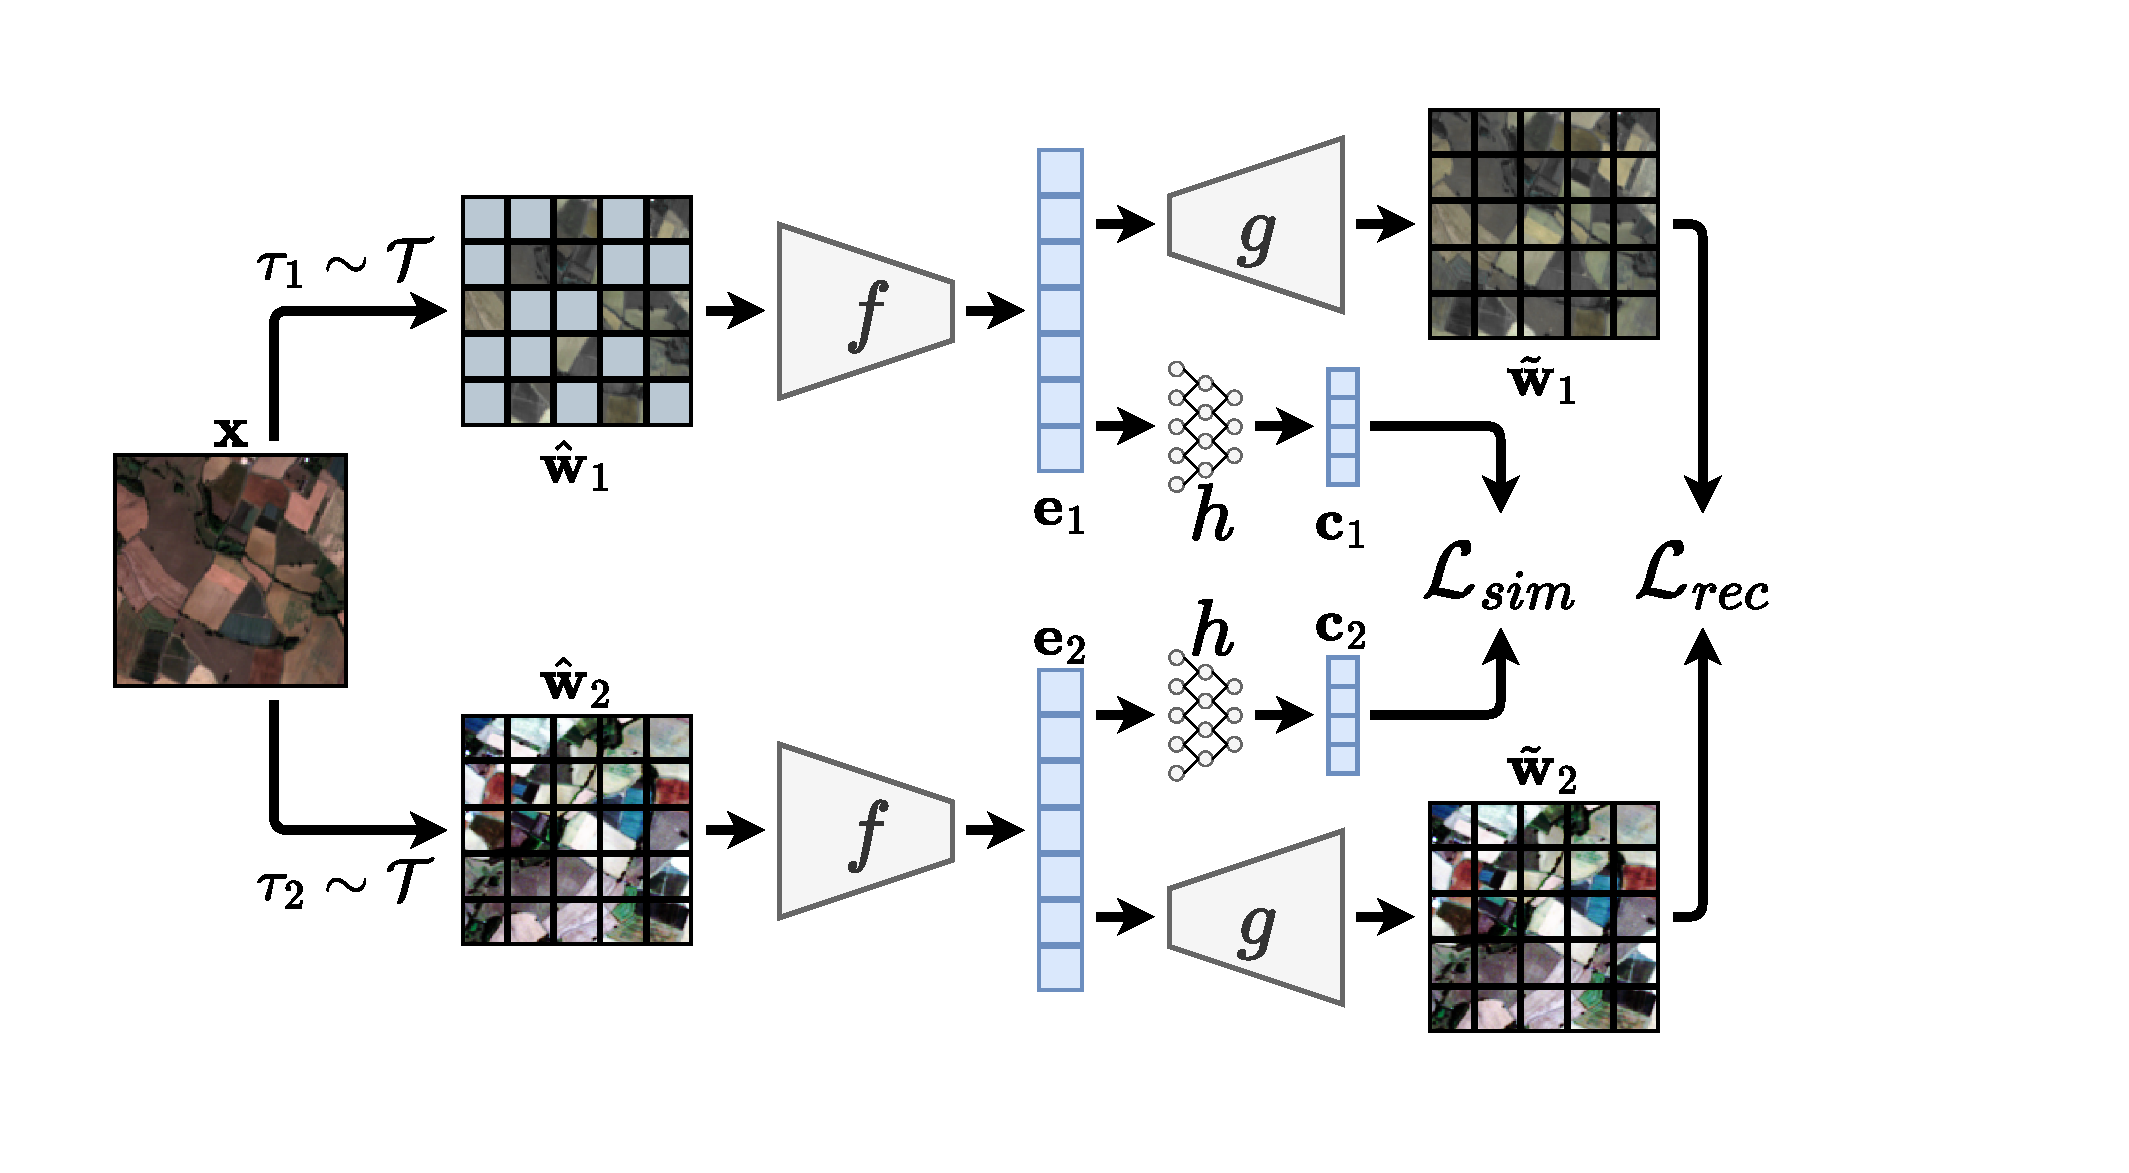
\includegraphics[clip,trim=0.75in 0.45in 2.2in 0.45in,scale=\figscale]{figures/3_theoretical_background/ssl/masked_image_modeling_similarity.pdf}
    \label{fig:ssl_mim_sim}
\end{figure}

\subsection{Semi-Supervised Hybrid Techniques} \label{sec:ssl_semi}

\fromsurvey{A very small area with few published works seeks to combine characteristics of semi-supervised learning with self-supervised learning, based on the hypothesis that \ac{SSL} can benefit from a small number of labeled samples. For this, strategies are used in which the \ac{SSL} pretext task on unlabeled data is performed during finetuning for the downstream task, in a semi-supervised fashion. Following this strategy, \cite{zhai2019s4l} then proposed the \Acf{S4L} method that classifies two augmentations of an image labeled with CELoss, and predicts transforms for these two augmentations added to two more from the unlabeled dataset, achieving the best performance in \ac{OA} on the ILSVRC-2012 Dataset, although comparisons with other methods are lacking. Few methods in this family have been used in \ac{RS}. \cite{singh2018self} used rotation prediction to aid classification, combining the two losses into a so-called Mixup Loss. The results were slightly better using this method, especially considering that rotation prediction in satellite images is quite complex since the directions in the images do not contain much semantic meaning.}
\section{Confidence Estimation and Anomaly Rebuttal}
\label{sec:conf_contextualization}

The use of \ac{DL} models in critical applications - such as autonomous driving, medical diagnosis, and, in the context of this work, large-scale agricultural monitoring - makes the reliability of these models a primary concern. It is not enough to simply search for models with high evaluation metrics; it is essential that such models be capable of assessing the reliability of their own predictions and identifying when a prediction is subject to significant uncertainty.

Historically, the standard approach to estimating the confidence of a classification model has been to use Maximum Class Probability (MCP), obtained directly from the softmax layer of the network, which is usually the last layer of a classification Deep Neural Network. However, the literature points out that MCP has significant conceptual flaws for confidence prediction. The main problem lies in the fact that modern neural networks are overconfident~\citep{NEURIPS2021_61f3a6db,pmlr-v162-wei22d}, assigning high probabilities even to incorrect predictions. This results in considerable overlap in the confidence distributions between hits and misses, making the raw use of network outputs poor confidence rankings.

\cite{corbiere2019addressing} proposes ConfidNet, an auxiliary neural network that estimates the reliability of a classification model's predictions, proposing the use of True Class Probability (TCP) as a target metric to distinguish failures, since the output of the last layer tends to be overconfident, even in incorrect predictions. In terms of methodology, ConfidNet is trained on the feature extraction layers of an already trained classifier, whose weights are kept frozen during the initial phase. Subsequently, the backbone of the original classifier is copied and its weights are fine-tuned together with the auxiliary confidence prediction network. The network minimizes an MSE calculated between the confidence predicted by ConfidNet and the probability that the original classifier assigned to the ground truth of that specific sample. As for the network architecture itself, it consists of linear layers with ReLU activation, ending with a sigmoid activation to ensure that the output is in the range of 0 and 1. This technique can be applied to any classifier network and will therefore be used as a baseline in this work.

While traditional classification assumes a closed set scenario, where all possible classes are known during training, the \acf{OSR} scenario, i.e., open set, assumes that the model must correctly classify known classes while identifying samples belonging to unknown classes~\citep{10582552}. \ac{OSR} techniques can be adapted to the confidence problem by treating incorrect predictions as anomalies or outliers in the model's embedding space. In this context, \acf{GeMOS}~\citep{vendramini2021opening} proposes a plug-and-play framework that couples a \ac{GMM} per predicted class on the embeddings of the network's intermediate layers extracted by a supervised \ac{CNN} trained on a closed set, with the training of the \ac{GMM}s limited to the training samples for which the network made correct predictions. During inference, the model calculates a likelihood score that indicates how well a sample fits the distribution of the predicted class, where low likelihood values suggest that the sample is an anomaly (or a classification error). Similarly, \cite{10418501} also suggests using \ac{GMM}s to model the distribution of embeddings, but using superpixels for \ac{OSR} in semantic segmentation.

\begin{figure}[ht!]
\centering
\caption{Comparison between closed set and open set classification.}
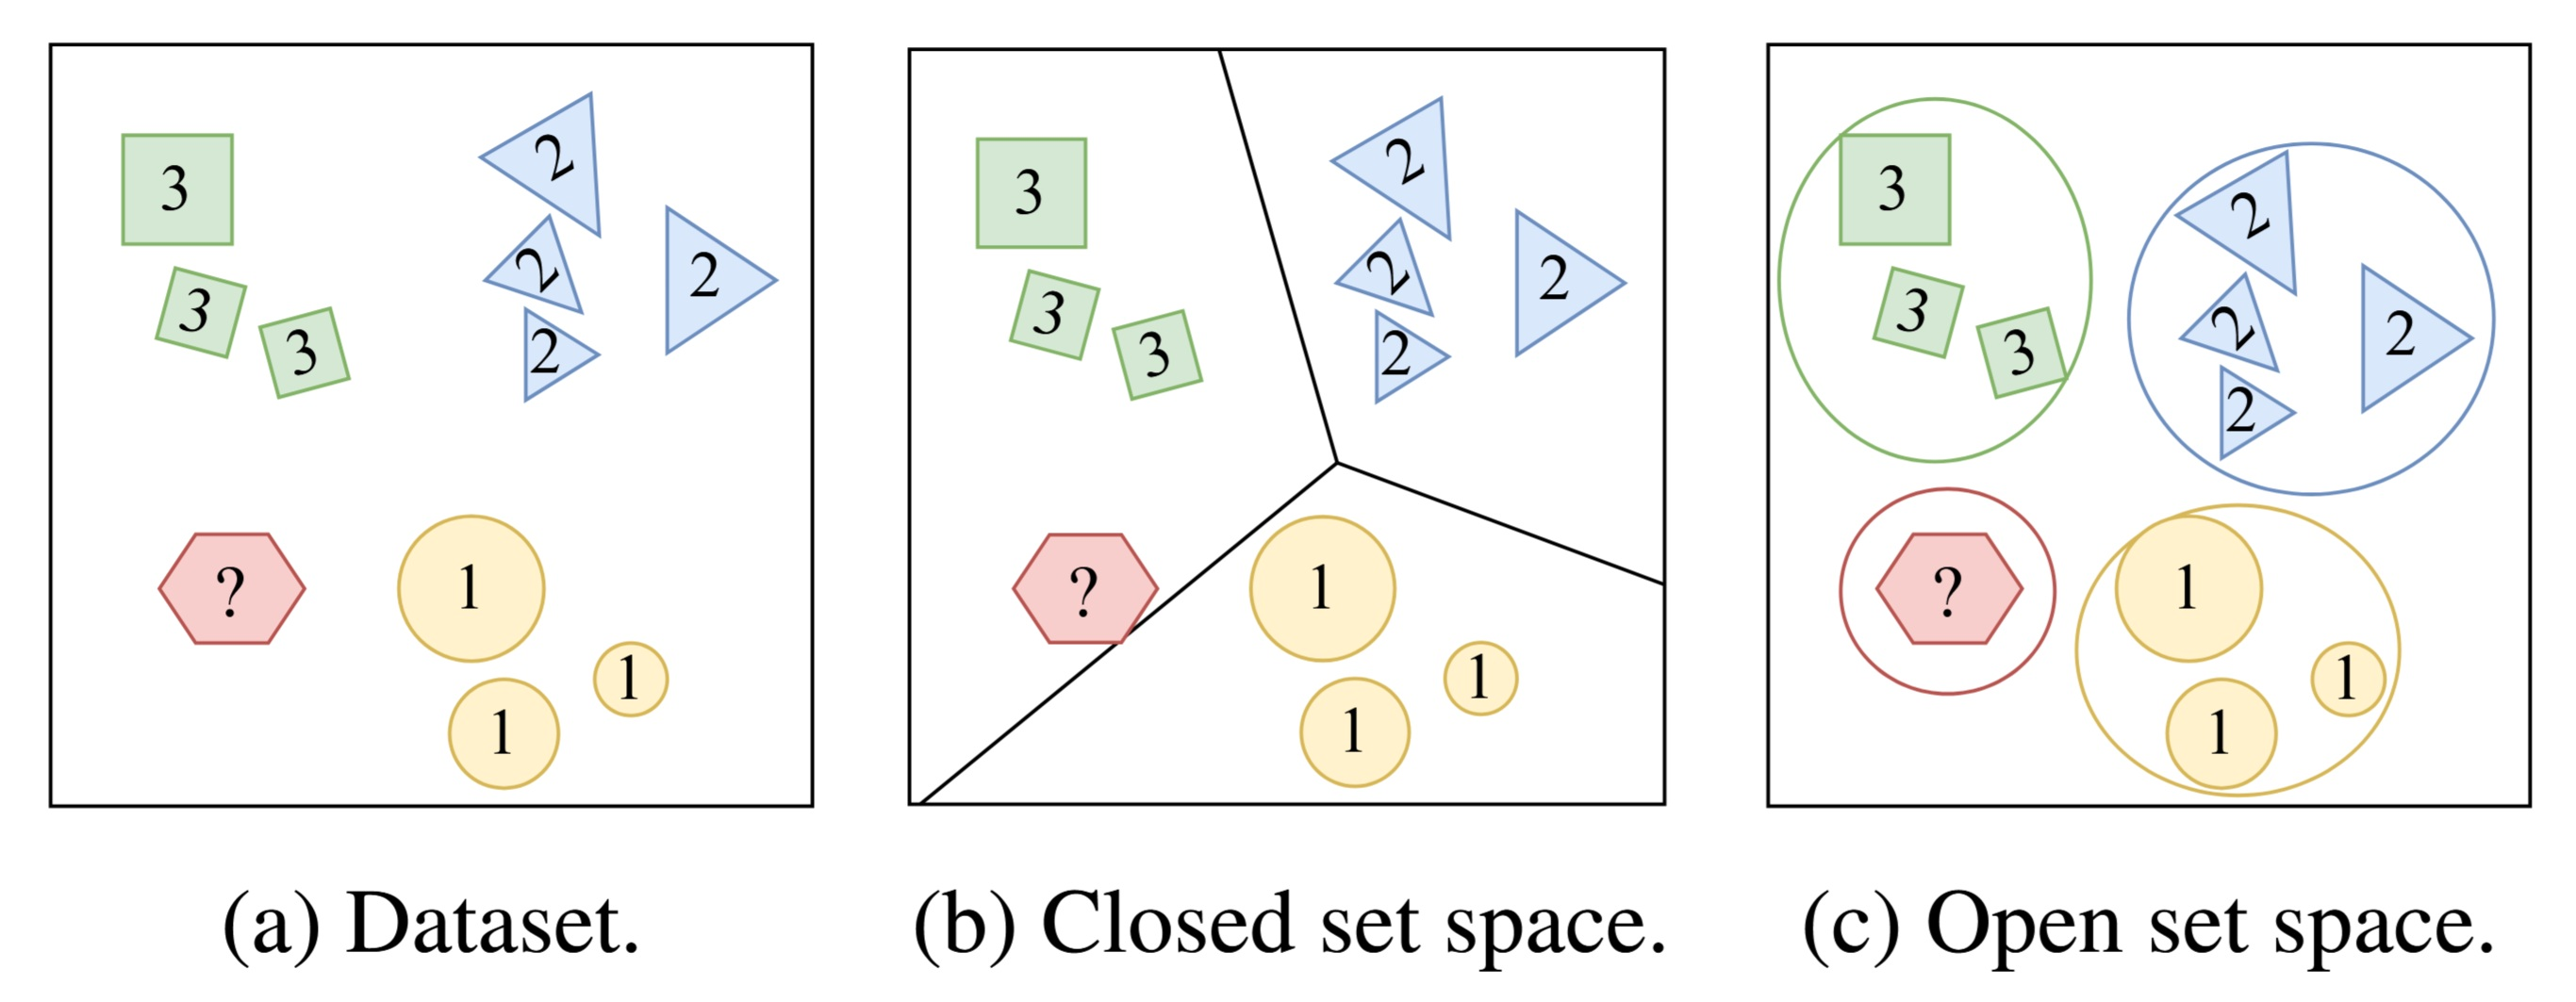
\includegraphics[width=0.95\linewidth]{figures/3_theoretical_background/gemos.jpg}
\fignote{One should notice that, in Closed Set (b) the sample ``?'', from a new class, would be classified erroneously as class 3. In Open set (c), the sample would be classified as an ``unknown'' class - Adapted from \cite{vendramini2021opening}}
\label{fig:osr}
\end{figure}

In addition to generative models on embeddings, other techniques seek semantic consistency by reconstructing the input data. The Conditional Reconstruction for Open-set Semantic Segmentation (CoReSeg) method~\citep{9897407} uses a conditional reconstruction approach, where the network attempts to reconstruct the input image only on known classes, which are those present in the training dataset. The premise is that objects of known classes will be well reconstructed, while unknown objects or classification errors will result in a high reconstruction error.